% Consolidated single manuscript: prediction, impact analysis, and
% mitigation in one document (technical paper + prediction companion merged,
% September 2026). Figures reuse the pipeline's own chart files
% (figures/figure_*.png, figures/supplemental/s*.png) plus exhibits generated
% from the same tables (figures/pred_*.png); all tables transcribe the
% September 2026 pipeline run (tables/table_*.csv, tables/pred_*.csv) rounded
% for readability --- see the pipeline's Table 8.6 for provenance.
% Compile from article/: pdflatex this file twice.
\documentclass[11pt,a4paper]{article}
\usepackage[margin=1in]{geometry}
\usepackage{amsmath,amssymb,booktabs,array,graphicx,xurl,hyperref}
\usepackage[table]{xcolor}
\usepackage{natbib}
\usepackage[section]{placeins}
\usepackage{enumitem}
\usepackage[font=small,labelfont=bf,labelsep=period,justification=raggedright,singlelinecheck=false]{caption}
\hypersetup{colorlinks=true,linkcolor=blue,citecolor=blue,urlcolor=blue,
pdftitle={Circular Capital in the Artificial Intelligence Stack: A Game-Theoretic Analysis of Market Power, Financial Fragility, and Welfare},
pdfauthor={Anonymous}}
\setcitestyle{authoryear,round}
\setlength{\bibhang}{0.5in}
\graphicspath{{figures/}}
% Pipeline-fed values: Table 8.7 intervals render from code output
% (generated_a8_intervals.tex, rewritten every ai_ecosystem_model run).
% GENERATED by StructuralEstimationAnalyzer.write_tex_macros -- do not edit.
% Values render Table 8.7 (table_8.7_structural_estimation.csv);
% the ai_ecosystem_model stage rewrites this file every run.
\newcommand{\AeightCapex}{[0.35, 2.63]}
\newcommand{\AeightHhi}{[0.10, 1.67]}
\newcommand{\AeightCirc}{[0.74, 3.00$+$]}
\newcommand{\AeightExub}{[0.00$+$, 1.04]}

\setlength{\parskip}{0.5em}
\rowcolors{2}{gray!10}{white}
% Whitespace control: many large floats share pages with text, so tighten
% float spacing and let top/bottom areas fill more aggressively.
\setlength{\textfloatsep}{12pt plus 2pt minus 2pt}
\setlength{\abovecaptionskip}{6pt}
\renewcommand{\textfraction}{0.07}
\renewcommand{\topfraction}{0.93}
\renewcommand{\bottomfraction}{0.9}
\setcounter{topnumber}{3}
\setcounter{bottomnumber}{3}
\title{Circular Capital in the Artificial Intelligence Stack:
A Game-Theoretic Analysis of Market Power, Financial Fragility, and Welfare}
\author{Anonymous for double-blind review}
\date{}
\begin{document}
\maketitle
\begin{abstract}
\noindent The 2024--2026 artificial-intelligence investment boom shows the
financing structure behind modern round-trip busts: dense,
committed circular capital in which upstream investment returns
as contracted compute spend, measured at \$675.40 billion across 17
committed edges. It concentrates burst incidence upstream.
Bubble conditions score $\sim$83\% at frontier labs (Foundation Models),
where private valuations detached furthest from capturable revenue.
Credit markets now charge for stack leverage (single-name CDS
at a record 215bp; a BBB- downgrade). Six solved bilateral games
yield aggregate deadweight loss of \$416.77 billion
at 71.28\% efficiency, with non-cooperation binding in the Hardware--Cloud
game. A severe burst destroys $\sim$\$239 billion of Hardware value and
$\sim$\$133 billion of Cloud value first, costing the US economy
$\sim$\$139 billion ($\sim$0.45\% of GDP) through capex and wealth channels.
The chain is mechanical: signed circular contracts trap value in the
Hardware--Cloud game, the trap fixes the loss order, and the order survives
16 extremes and 300 joint draws. Run blind on 2008
inputs, the same modules recover the historical loss order
(thirteen of fourteen verdicts). The dollar figures size remedies;
the ranking is the forecast. By benefit--cost ratio,
disclosure and lending caps come first. Three stated observables would retire
the call.
\medskip

\noindent\textbf{Keywords:} artificial intelligence; financial bubbles;
circular dealing; vendor financing; game theory; financial stability.
\medskip

\noindent\textbf{JEL codes:} D43, G01, G12, G14, L13, L41, E44, O33.
\end{abstract}

\section{Introduction}
This paper converts a measured financing structure into a dated,
testable prediction: an AI-asset repricing is likely while the current
committed spend cycle runs; its losses will land first on Hardware, then
Cloud, then frontier labs, then apps; and the severe case costs the US
economy roughly \$100--150~billion. Section~\ref{sec:prediction} states
that forecast as eight numbered claims, each with an assessed likelihood
(or an explicit abstention, P8) and a pointer to the observable that would
overturn it. The remaining
sections supply the evidence (Sections~\ref{sec:capital}--\ref{sec:contagion}),
the record of stress testing and historical validation
(Sections~\ref{sec:robustness}--\ref{sec:backtest}), and the investment and
policy implications (Sections~\ref{sec:triggers}--\ref{sec:policy}).

The argument is a five-link chain. \textbf{Measurement:} \$675.40~billion
of committed circular capital read off signed contracts
(Section~\ref{sec:capital}). \textbf{Mechanism:} six solved games show
non-cooperation binds in exactly one cell --- Hardware versus Cloud
(Sections~\ref{sec:games}--\ref{sec:core}). \textbf{Incidence:} the trap
fixes the burst order, with formation worst where private marks detached
furthest (Sections~\ref{sec:bubble}--\ref{sec:burst}). \textbf{Validation:}
the order survives sixteen extremes and 300 joint draws, and the same
modules recover the 2008 loss order and the 2001 telecom mechanism
(Sections~\ref{sec:robustness}--\ref{sec:backtest}). \textbf{Action:}
triggers plus remedies sequenced by benefit--cost ratio
(Sections~\ref{sec:triggers}--\ref{sec:policy}). Throughout,
\emph{rankings} are the high-confidence claims; \emph{dollar figures} mark
scenario scale for sizing remedies.

\section{Central Forecast: Repricing Likelihood, Loss Incidence, and Macroeconomic Cost}\label{sec:prediction}
This paper makes a prediction with three parts. \textbf{First}, an AI-asset
repricing is likely while the current committed spend cycle runs: the
conditions that have preceded every modern round-trip bust --- dense
reciprocal financing, private marks detached from capturable revenue, and
credit markets starting to charge for leverage --- are all present at once.
\textbf{Second}, the damage has a fixed address: Hardware first
($\sim$\$239B), Cloud second ($\sim$\$133B), frontier labs third
($\sim$\$85B), app companies last ($\sim$\$21B), because contracts, not
sentiment, decide where losses land. \textbf{Third}, the US GDP cost of the
severe case is $\sim$\$139B ($\sim$0.45\%), composed of canceled tech
investment ($\sim$\$120B) plus the wealth effect of falling equities
($\sim$\$19B).

What this paper does \emph{not} predict is a date. Timing belongs to funding
rounds, credit events, and capex guidance --- the triggers of Section~\ref{sec:triggers} ---
not to models. Everything else here is a measured claim, not a scenario
sketch: the capital structure is read off contracts, the binding constraint
is proved in solved games, and the resulting incidence ranking is the same
order that survives every stress battery and transfers to 2008. The result
is a standing warning with an address book: it tells you what breaks, in
what order, at roughly what scale, and what to do before it happens.

\emph{How seriously to take each claim.} Each prediction carries a
\textbf{likelihood} (author-assessed probability on the fixed scale in
Table~\ref{tab:likelihood-scale}) and a \textbf{confidence} grade (quality
of evidence). Model vote-shares measure \emph{robustness} and formation
scores \emph{vulnerability} --- neither is an event probability.

\begin{table}[htbp]
\centering
\caption{Likelihood scale for author-assessed probabilities. Used only in the registry below; nowhere else in the paper does a percent sign denote an event probability.}
\label{tab:likelihood-scale}
\begin{tabular}{lc}
\toprule
Wording & Assessed probability \\
\midrule
Very likely & 85--95\% \\
Likely & 65--80\% \\
More likely than not & 50--65\% \\
Toss-up & $\sim$50\% \\
Unlikely & below 35\% \\
\bottomrule
\end{tabular}
\end{table}

\begin{table}[htbp]
\centering
\caption{Prediction registry: every claim, its likelihood, its evidence grade, and what retires it.}
\label{tab:registry}
\begin{tabular}{l>{\raggedright\arraybackslash}p{4.4cm}>{\raggedright\arraybackslash}p{2.7cm}c>{\raggedright\arraybackslash}p{3.0cm}}
\toprule
ID & Claim & Likelihood & Confidence & Overturned by \\
\midrule
P1 & AI-asset repricing before the committed spend cycle exhausts itself & Likely ($\sim$65\%) & Medium & Validation tests 1--2 \\
P2 & \emph{Conditional on a severe burst,} losses rank Hardware $>$ Cloud $>$ labs $>$ apps & Very likely ($\sim$90\%) & High & Test 3 (ranking flips) \\
P3 & Severe GDP cost lands near \$100--150B ($\sim$0.3--0.5\%), mostly via canceled capex & More likely than not ($\sim$55\%) & Medium & A burst with no capex cut \\
P4 & Frontier-lab funding stress is the nearest trigger & Likely ($\sim$70\%) & Medium & A first break elsewhere (Sec.~\ref{sec:triggers}) \\
P5 & Labs carry the highest bubble vulnerability (formation rank FM first) & More likely than not ($\sim$60\%) & Medium & Formation rank flips (65\% joint agreement) \\
P6 & Round two is small ($\sim$\$15B), mostly on labs ($\sim$\$13.9B of $\sim$\$15.2B) & More likely than not ($\sim$60\%) & Medium & Collateral fire sale (Sec.~\ref{sec:contagion}) \\
P7 & Disclosure first, lending caps second is the optimal remedy sequence (caps still rank first by BCR) & Likely ($\sim$70\%) & Medium & BCR rank reversal (Sec.~\ref{sec:policy}) \\
P8 & Any calendar date for the repricing & --- (unassigned) & Low & --- (no date predicted) \\
\bottomrule
\end{tabular}
\end{table}

Read P2 as written: \emph{conditional} --- $\sim$90\% on the ranking
\emph{given} a severe burst, whose occurrence is P1's $\sim$65\%. Jointly
``a severe burst with Hardware first'' sits near 60\%: a standing warning
with an address book, not a forecast.


\section{Analytical Approach: Contractual Exposure as the Forecasting Primitive}\label{sec:foundation}
Most bubble calls argue about prices. This one argues about \emph{plumbing}:
the \$675.40B of committed round-trip financing, across 17 booked deals,
that wires the AI stack into a single fate-sharing machine. When company A
invests in company B and B contractually spends the money back at A, two
balance sheets become one balance sheet wearing two logos. Prices can then
stay high for good reasons (real revenues: NVIDIA's record \$57.0B quarter, Q3 FY2026)
while the financing underneath stays fragile. That split --- real revenues,
fragile financing --- is what makes a burst prediction possible without a
price prediction: you do not need to know when enthusiasm fades, only where
the contracts point when it does. The machinery is a single Python
pipeline of 35 classes covering data validation, market structure, solved
games, welfare accounting, bubble diagnostics, and valuation, gated end to
end by 364 tests.

Why this toolkit and not price charts. Traditional bubble models study
anonymous markets through prices, sentiment, or aggregates; the AI stack is
the opposite --- a handful of giants negotiating bespoke bilateral
contracts --- so the tools model the plumbing directly. \emph{Game theory}
solves each pairwise negotiation for its stable outcome, exposing the one
gridlocked cell. The \emph{Herfindahl--Hirschman Index} (the DOJ
concentration screen, highly concentrated above 2,500) quantifies the
chokepoint: at 3,851, no diversified fringe exists to absorb a failure.
\emph{Saltelli global sensitivity analysis} (the variance-decomposition
workhorse of physics and climate modeling) then checks which input actually
drives fragility: shared circular capital scores a total-order index of
0.99, confirming the prediction emphasizes the variable the system is most
sensitive to.

\section{Literature Review: Bubbles, Platforms, and Fragility}\label{sec:literature}
This prediction does not start from zero. Five strands of published research
supply its tools, its benchmarks, and its warnings; this section states each
in one paragraph, with pointers for readers who want the originals. Full
references sit in the References list, in APA style.

\emph{1. How economists spot bubbles.} The standard statistical toolkit hunts
explosive price paths: \citet{phillips2011} built the SADF test that
date-stamps when exuberance starts and collapses, and
\citet{phillips2015} generalized it to multiple bubbles. The dot-com
precedent --- world-changing technology alongside prices far above eventual
cash flows --- is documented by \citet{ofek2003}, while \citet{greenwood2019}
show such run-ups predictably end in crashes.
Takeaway for this paper: price tests tell you \emph{whether} something looks
explosive; they cannot tell you \emph{where the losses land}. The financing
graph modeled here answers the second question, which is why the two
approaches complement rather than compete.

\emph{2. What AI does to the economy.} The economics-of-AI program
\citep{agrawal2018, agrawal2019} now measures real generative-AI
productivity gains \citep{brynjolfsson2025, noy2023} against slow
general-purpose-technology payoffs \citep{brynjolfsson2021, david1990},
while macro watchdogs flag AI-correction risk, big-tech leverage, and
supply-chain funding complexity \citep{imf2026b, imf2026, bis2026}.
Takeaway: the revolution is real \emph{and} the financing is fragile.

\emph{3. Why platforms lock customers in.} Cloud bundling follows the
information-goods logic of \citet{shapiro1999} and \citet{bakos2000};
switching costs and network effects are surveyed by \citet{farrell2007};
sunk-cost market structure by \citet{sutton1991}; semiconductor competition
by \citet{scherer1990}. On policy, the Digital Markets Act \citep{eu2022},
the digital-era competition report \citep{cremer2019}, vertical-stack
analysis \citep{hagiu2025}, the antitrust-paradigm literature
\citep{baker2019}, and data-portability economics \citep{kramer2020} shape
the remedy menu, while the FTC documents investment capital bundled with
cloud spend \citep{ftc2025}. Takeaway: lock-in theory predicts exactly the
\$142.62B switching-cost envelope this paper measures --- the oldest
literature here correctly calls the largest waste category. The classic
monopoly-waste benchmark is \citet{harberger1954}, and the reason fixing one
broken margin can backfire elsewhere is \citet{lipsey1956}.

\emph{4. Vendor financing and fire sales.} Round-trip financing has a known
pathology (telecom vendors lending to their own buyers), and the fire-sale
mechanic --- homogeneous collateral worth less together than apart --- is
formalized by \citet{shleifer1992}. The cascade engine in this paper is the
DebtRank method of \citet{battiston2012}. Takeaway: every moving part of the
contagion story is borrowed from established work; the novelty is wiring
them into one stack with measured exposures.

\emph{5. Concentration and hype measurement.} AI markets concentrate through
fixed training costs and size advantages even without misconduct
\citep{korinek2025}; scale, GDP, and valuation anchors come from
institutional-grade public sources \citep{iea2026, idc2026, pwc2026,
bea2026, cbo2022, damodaran2026}, listed to the row in the pipeline's
110-row register.

\section{Measurement of Circular Capital: Scale and Composition}\label{sec:capital}
Seventeen committed deals, each traced to primary reporting and re-verified
in September 2026, put \$675.40B of circular capital on the books
(\$1,188.33B tracked including two memo rows); the largest rows are a
\$249.20B aggregate GPU-supply exposure and a \$105B NVIDIA credit
guarantee (Table~\ref{tab:01-largest-committed-circular-exposures}).
Parked \emph{outside} the booked total, exactly as they should be:
Google's \$30B conditional tranche, Amazon's \$20B, an NVIDIA tranche of up
to \$10B, decade-horizon reverse spends, the
\$500B six-platform MOU facility (aspiration, not a contract), and the
\$12.93B NVIDIA--Hugging Face acquisition (a purchase price for control,
with no reverse-spend leg).

\begin{table}[htbp]
\centering
\caption{Largest committed circular exposures (\$B). Full 19-row frame in the pipeline's validated deal ledger (pipeline Table~3 series).}
    \label{tab:01-largest-committed-circular-exposures}
\begin{tabular}{lr}
\toprule
Exposure & Committed \\
\midrule
Aggregate GPU-supply exposure & 249.20 \\
NVIDIA \$105B Ohio credit guarantee & 105.00 \\
Lambda + Nscale compute commitment & 80.00 \\
Fluidstack compute & 50.00 \\
SpaceX Colossus & 45.00 \\
AWS cloud agreement (OpenAI) & 38.00 \\
Azure purchase (Anthropic) & 30.00 \\
CoreWeave contract (Meta) & 14.20 \\
Microsoft--OpenAI / Amazon--Anthropic & 13.00 each \\
\midrule
\textbf{Committed total (17 edges)} & \textbf{675.40} \\
Tracked total (19 rows) & 1,188.33 \\
\bottomrule
\end{tabular}
\end{table}



Prediction consequence: one row (GPU supply, 36.9\%) and one pair
(Hardware--Cloud) dominate the frame, and Hardware (54.7\%) plus Cloud
(42.2\%) own 97\% of the 3,851-point concentration index --- so the burst
has a chokepoint. More than three-quarters of the frame is procurement
(propagating at face in DebtRank), while the 15.5\% guarantee layer is
contingent: small in the base case, outsized in the severe one.

\section{Strategic Interaction: Six Bilateral Games and the Scope for Cooperation}\label{sec:games}
The core game is the prediction's engine, but the other five set its
boundaries. Each row below gives the stable outcome, the best-joint
outcome, the trapped value, and the payment that would unlock it.

\begin{table}[htbp]
\centering
\caption{All six games: stable vs.\ best-joint welfare (\$B).}
    \label{tab:02-all-six-games-stable}
\begin{tabular}{lcccc}
\toprule
Game & Nash & Joint max & Trapped & Transfer to unlock \\
\midrule
HW--Cloud & 1,094.8 & 1,153.4 & 58.6 & 176.0 (HW to Cloud) \\
HW--Foundation & 671.3 & 876.9 & 205.6 & 46.7 (HW to FM) \\
HW--Wrappers & 609.0 & 856.1 & 247.0 & 18.7 (HW to Wrappers) \\
Cloud--Foundation & 604.1 & 745.4 & 141.2 & 46.3 (Cloud to FM) \\
Cloud--Wrappers & 544.3 & 725.0 & 180.7 & 18.7 (Cloud to Wrappers) \\
FM--Wrappers & 142.5 & 177.1 & 34.6 & 1.1 (FM to Wrappers) \\
\midrule
\textbf{Diagnostic sum} & & & \textbf{867.8} & \textbf{307.4} \\
\bottomrule
\end{tabular}
\end{table}

Three prediction readings. \emph{First}, the largest trapped value
(\$247.0B, Hardware--Wrappers) needs the smallest key (\$18.7B): the
cheapest cooperation in the stack is also among the most valuable, which is
where a negotiated settlement would start. \emph{Second}, every unlock
payment flows upstream-to-downstream, so in a crisis the kill chain runs
through whoever refuses to pay --- watch Hardware's and Cloud's willingness
to compensate, not the labs'. \emph{Third}, the core game's \$176.0B price
tag on a \$58.6B gain is the worst ratio in the stack: the most important
cooperation is the least likely to happen voluntarily, which is why it needs
regulation rather than hope. (The \$867.8B sum multi-counts shared players
across pairs; the \$416.77B top-down bound, not this sum, sizes policy.)


Stability sharpens the timing logic (Table~7.4): four of six games are
stable loss pockets ($\geq$80\% Nash reproduction), while the core game
reproduces at 64.7\% --- the modal outcome, not a certainty. P2's
$\sim$90\% burst ranking follows contracts rather than equilibria, so even
draws where the core game flips leave the loss address unmoved.

\section{The Binding Constraint: Non-Cooperation in the Hardware--Cloud Game}\label{sec:core}
Six pairwise standoffs were solved. All six trap value absent cooperation,
but only one binds the prediction: Hardware vs.\ Cloud. Chipmakers stay
open while clouds stay locked
in --- neither side wants to move alone --- trapping \$58.6B that
cooperation would unlock (94.9\% efficient). That single stuck relationship,
sitting on the largest contract base in the stack, is the structural reason
a repricing becomes a loss rather than a shrug.

\begin{table}[htbp]
\centering
\caption{The core Hardware--Cloud game (\$B). The stuck cell is the selected equilibrium; the best-joint cell is Nash too --- payoff- and risk-dominant --- but unselected, so persistence of the inferior cell is a lock-in story, not an incentives story.}
    \label{tab:03-the-core-hardwarecloud-game}
\begin{tabular}{lcc}
\toprule
 & Cloud: Open & Cloud: Locked (Nash) \\
\midrule
Hardware: Open (Nash) & --- & 487.9 + 606.8 = 1,094.8 \\
Hardware: Walled (Pareto) & 722.5 + 430.8 = 1,153.4 & --- \\
\bottomrule
\end{tabular}
\end{table}


Two audits sharpen the reading: the efficient outcome is payoff- and
risk-dominant (Table~3.6) yet unselected --- lock-in, not incentives, holds
the inferior cell --- and cooperation is sustainable without transfers in
three of six games including the core, while the three lab games cannot
sustain it at any patience level (Table~3.7).

\section{Welfare Analysis: Decomposition of Deadweight Loss}\label{sec:welfare}
The stuck games waste \$416.77B in total, itemized in Table~\ref{tab:04-waste-by-source-b}.
The prediction-relevant fact is the ordering, which survives every stress test:
lock-in first (\$142.62B), distorted R\&D second (\$106.97B). Remedies aimed
anywhere else are aimed at smaller problems.


\begin{table}[htbp]
\centering
\caption{Waste by source (\$B). Order first, levels second.}
    \label{tab:04-waste-by-source-b}
\begin{tabular}{lr}
\toprule
Source & Loss \\
\midrule
Switching costs (lock-in) & 142.62 \\
Innovation distortion & 106.97 \\
Quality degradation & 71.31 \\
Coordination failures & 60.01 \\
Monopoly pricing & 35.86 \\
\midrule
\textbf{Total} & \textbf{416.77} \\
\bottomrule
\end{tabular}
\end{table}


\section{Bubble Vulnerability Assessment by Archetype}\label{sec:bubble}
Bubble-condition scores (vulnerability ratings from a scenario-calibrated
model, not measured probabilities; bands plotted below, drivers in the
\texttt{pred\_E} ledger) peak exactly where round-tripping is densest.

Prediction consequence: monitor frontier-lab funding rounds as the leading
indicator. Each mega-round at a higher valuation re-prices every adjacent
private mark at once. Anthropic at \$965B, Databricks near 905x earnings,
and xAI at 400x revenue have the furthest to fall.

\begin{figure}[htbp]
\centering
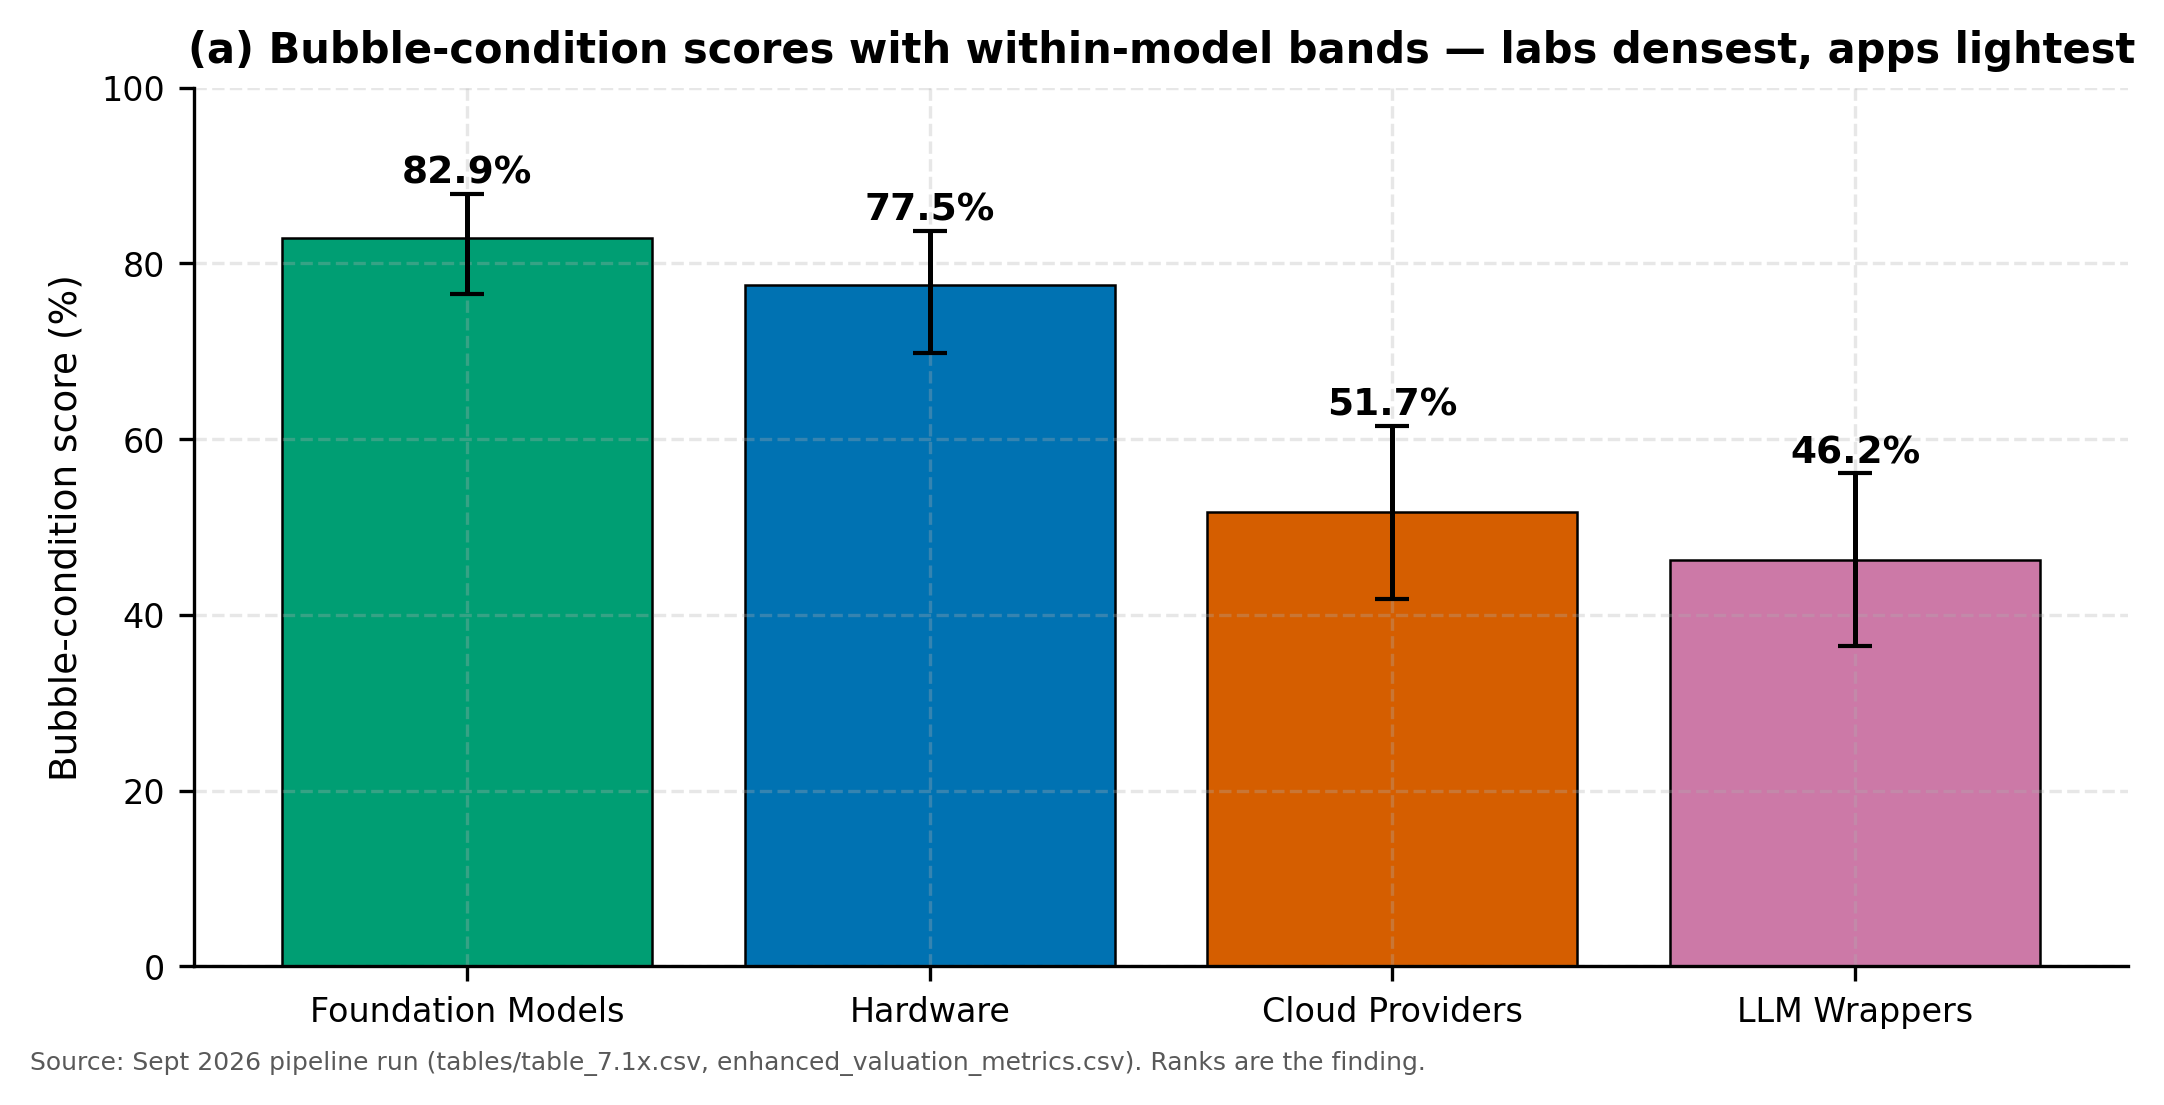
\includegraphics[width=\textwidth,height=0.82\textheight,keepaspectratio]{pred_formation_bands.png}
\caption{Bubble-condition scores with within-model robustness bands. The gap that matters is the top-two vs.\ bottom-two split: round-tripping density, not hype, separates them --- Wrappers carry maximum exuberance (1.0) yet score lowest (46.2\%) because their circular exposure is near zero (0.027).}
    \label{fig:10-bubblecondition-scores-with-withinmodel}
\end{figure}

\begin{table}[htbp]
\centering
\caption{Bubble-score driver decomposition (logit inputs; Table~7.10). Circular exposure dominates by construction (weight 1.6); exuberance alone cannot lift a score.}
    \label{tab:06-bubblescore-driver-decomposition-logit}
\begin{tabular}{lccccc}
\toprule
Archetype & Circ. & Capex & HHI sh. & Exub. & Score \\
\midrule
Foundation Models & 0.80 & 0.70 & 0.10 & 1.00 & 82.9 \\
Hardware & 0.40 & 0.90 & 0.46 & 0.83 & 77.5 \\
Cloud Providers & 0.23 & 0.60 & 0.40 & 0.09 & 51.7 \\
LLM Wrappers & 0.03 & 0.20 & 0.04 & 1.00 & 46.2 \\
\bottomrule
\end{tabular}
\end{table}

Driver reading: Hardware trails labs on circular exposure (0.40 vs.\ 0.80)
despite leading three other pillars; Cloud's near-zero exuberance (0.09)
is why the credit tripwire starts at leveraged Cloud-adjacent names
(Section~\ref{sec:contagion}). Full ledger: \texttt{pred\_E\_formation\_drivers.csv}.

Uncertainty propagates three ways: stated bands ($z\pm0.4$), one-at-a-time
quartering through quadrupling (10/16 formation-order, 16/16 burst-order),
and a 300-draw joint check (seed 7): formation exact-match 65\%
($\tau=0.88$, labs top 90\%), burst exact-match 100\% ($\tau=1.00$,
Hardware first throughout). Scores: \textbf{82.9\%} labs (76.5--87.9),
\textbf{77.5\%} Hardware (69.8--83.7), \textbf{51.7\%} Cloud (41.8--61.5),
\textbf{46.2\%} Wrappers (36.5--56.1) --- scenario-calibrated
vulnerability, not estimated event probabilities. Weights carry
structurally identified intervals (Table~8.7): capex \AeightCapex{}, HHI
\AeightHhi{}, circularity \AeightCirc{}, exuberance \AeightExub{}.

A second, independent screen agrees: the five-pillar classification
(Table~7.7) labels labs the sole ``Bubble risk'' (0.507), Hardware and
Wrappers ``Boom'' (0.408, 0.352), Cloud ``Buildout'' (0.317). Both screens
corroborate the registry; neither changes its likelihoods. Fragility and
instability coincide --- labs and apps least stable (0.38, 0.12),
infrastructure most (0.78, 0.75) --- yet the burst order runs opposite:
what breaks first in funding order breaks last in dollar order.

\section{Burst Incidence: Loss Ranking, Severity, and Macroeconomic Transmission}\label{sec:burst}
A severe scenario (70\% of circular capital impaired, 30\% AI-capex cut)
destroys value in the reverse order of the hype:

\begin{table}[htbp]
\centering
\caption{Severe-burst destruction by archetype (\$B): Hardware \$239.4B (50.1\%), Cloud \$132.7B (27.7\%), labs \$85.4B (17.9\%), Wrappers \$20.8B (4.4\%); shares sum to 100.1\% on rounding.}
    \label{tab:08-severeburst-destruction-by-archetype}
\begin{tabular}{lcr}
\toprule
Archetype & Loss & Rank \\
\midrule
Hardware & 239.4 & 1 \\
Cloud Providers & 132.7 & 2 \\
Foundation Models & 85.4 & 3 \\
LLM Wrappers & 20.8 & 4 \\
\midrule
\textbf{First-round total} & \textbf{478.3} & \\
Second reverberation round & 15.2 & \\
\bottomrule
\end{tabular}
\end{table}

The ranking is the most stress-tested claim in this paper: 16 of 16
one-at-a-time extremes, 100\% agreement across 300 joint draws, Hardware
first every time, replicated across seeds and noise screens. It holds
because inference still runs on someone's silicon and someone's cloud no
matter whose logo is on the model.

Direct-vs.-network split adds a second prediction inside the ranking:
Hardware's loss is 56\% direct (\textasciitilde\$133B of \$239.4B) --- it owns the
impaired contracts --- while Wrappers' loss is 97\% network (\$20.16B of
\$20.83B): apps are pure contagion victims with almost no direct exposure
(\$0.67B). Cloud splits evenly (\$67.85B direct, \$64.85B network); labs lean
direct (\$59.64B vs.\ \$25.75B). A burst that spares Hardware's contract book
but hits app revenues would flip the Wrappers row without moving the top
two --- one more reason the ranking's head is sturdier than its tail.

The valuation-vs.-contract paradox is the point, not a puzzle: frontier
labs score highest on bubble vulnerability (82.9\%) because private marks
detached furthest from revenue, yet Hardware absorbs the largest dollar
hit because it holds the contracts, the guarantees, and the capex. Screens
built on multiples would aim at the labs; the money says aim at the
toolmakers.

\emph{When, not just how much.} Formation scores convert into a burst-timing
window under a stated quarterly hazard: hazard equals formation probability
divided by a 12-quarter formation-to-burst lag (the 2005--2008 and
1999--2002 vintages both run about three years from dense formation to
burst), with median quarters to burst $\ln(2)/h$. The first-tip system clock
reads a median of 10.0 quarters from the September 2026 vintage (Q2'29),
set by Foundation Models at the same horizon; Hardware follows at
10.7 quarters (Q3'29), Cloud at 16.1 (Q4'30), Wrappers at 18.0 (Q2'31).
The honest uncertainty is the lag, not the band: varying it over 8--20
quarters spans Q3'28--Q1'31 at the system level, while the formation band
barely moves the median. Scenario arithmetic, not a forecast: move the
stated lag and every quarter moves with it. Machine-readable:
\texttt{pred\_G\_burst\_timing.csv}.

\emph{Why this timing, and what would change it.} The 10.0-quarter base is a
hazard clock, not a date prediction (P8 stays unassigned). Conditioning on
September-2026 evidence gives a conditional call at a median of 11.0 quarters (Q3'29), window Q4'28--Q2'31; any tripwire
tripping revokes the +1Q calm credit (median back to 10.0Q), and double
credit reaches 12.0Q (Q4'29). Machine-readable:
\texttt{pred\_L\_timing\_rationale.csv}.


Within-layer concentration (Table~7.1b) rules out the comforting story that
any single archetype is internally competitive: every layer screens
``highly concentrated'' (HHI 4,057--5,632), with the frontier-lab duo most
concentrated of all (5,283, Anthropic 61.9\%). There is no diversified
corner of the stack to hide in --- which is why the burst ranking is an
address book, not a hedge.

GDP transmission runs through two channels calibrated to US GDP
(\$30,767.1B): canceled tech investment (\$120.0B severe; \$40.0B mild) and
the equity-wealth effect at 4 cents on the dollar (\$19.1B severe; \$8.2B
mild) --- combined severe cost \$139.1B (0.452\% of GDP), mild \$48.2B
(0.157\%), no multiplier. The capex channel dominates in both states
(86\% severe, 83\% mild); wealth adds $\sim$\$4B per \$100B destroyed.
Portable rule: each \$100B of destroyed AI value
drags $\sim$\$4B of GDP through household wealth, plus the local capex-cut
share. Who holds that wealth loss --- and at what propensity to consume ---
is a retirement story: the uniform 4-cent assumption overstates the
aggregate drag while understating its concentration on 401(k) and pension
holders.

\section{Contagion Channels: Cascades, Collateral, and Credit}\label{sec:contagion}
Direct destruction is only round one. Full reverberation through the
committed deal graph --- the DebtRank cascade \citep{battiston2012} run to convergence --- adds \$15.2B more (concentrated in frontier labs), a
1.032 multiplier kept near one only by large equity buffers, not small
exposures. The 2008 analog lives in the collateral layer: homogeneous,
supplier-guaranteed GPU collateral correlates exactly when it must be sold.

\begin{table}[htbp]
\centering
\caption{Second-round cascade losses (\$B). First round: Table above.}
    \label{tab:09-secondround-cascade-losses-b}
\begin{tabular}{lr}
\toprule
Archetype & Second round \\
\midrule
Foundation Models & 13.86 \\
Cloud Providers & 1.27 \\
Hardware & 0.00 \\
LLM Wrappers & 0.07 \\
\midrule
\textbf{Total second round} & \textbf{15.20} \\
\textbf{Multiplier} & \textbf{1.032} \\
\bottomrule
\end{tabular}
\end{table}

Credit markets have started charging for exactly this structure: Oracle's
5Y CDS printed a record 215bp (implying $\sim$3.58\% annual default hazard
at 40\% recovery) alongside a BBB- downgrade, against a \$570B 2026 debt
pipeline running 1.43x one year of Big Four capex. The downgrade watchlist
follows the burst order --- Hardware first (\$239.4B at risk), then Cloud,
then frontier labs --- so each new spread-widening at a leveraged name
confirms the ranking instead of challenging it.

\section{Robustness and Sensitivity Analysis}\label{sec:robustness}
Predictions are only as good as their survival under attack. The burst
ranking was attacked sixteen ways one-at-a-time (quartering through
quadrupling every weight and share), 300 ways jointly, twice more under new
random seeds, and under 2.5\%, 5\% and 10\% measurement noise --- and never
moved. Monte Carlo reproduction holds at 64.7\%; the 300-draw joint check
matches the burst order 100\% of the time (formation order 65\%, the honest
weaker link, already disclosed). Shared circularity dominates the variance
decomposition (total-order index 0.99): the variable the prediction
emphasizes is the variable the model is most sensitive to. Structural
estimation (Table~8.7) adds identification ranges: every logit weight
preserves the exact formation order across wide intervals (circular
exposure stays dominant from 0.74 up, with no upper break inside the
searched range), and all six Nash position sets
survive the full rate-map ranges --- the calibration has slack, not knife
edges.

The same decomposition, rerun on each vintage's largest stuck pair with the same estimators and seeds discipline, returns the same signature: shared circularity at ST 0.97 in 2008 (Investors--Guarantors) and ST 0.96 in telecom (Incumbents--AltCarriers), top-tier in both. Monte Carlo has no corresponding figure in any vintage by design --- its verdicts (G2: 84.0\% 2008, 85.8\% telecom) live in the ledgers, where a number is the whole message.

\begin{figure}[htbp]
\centering
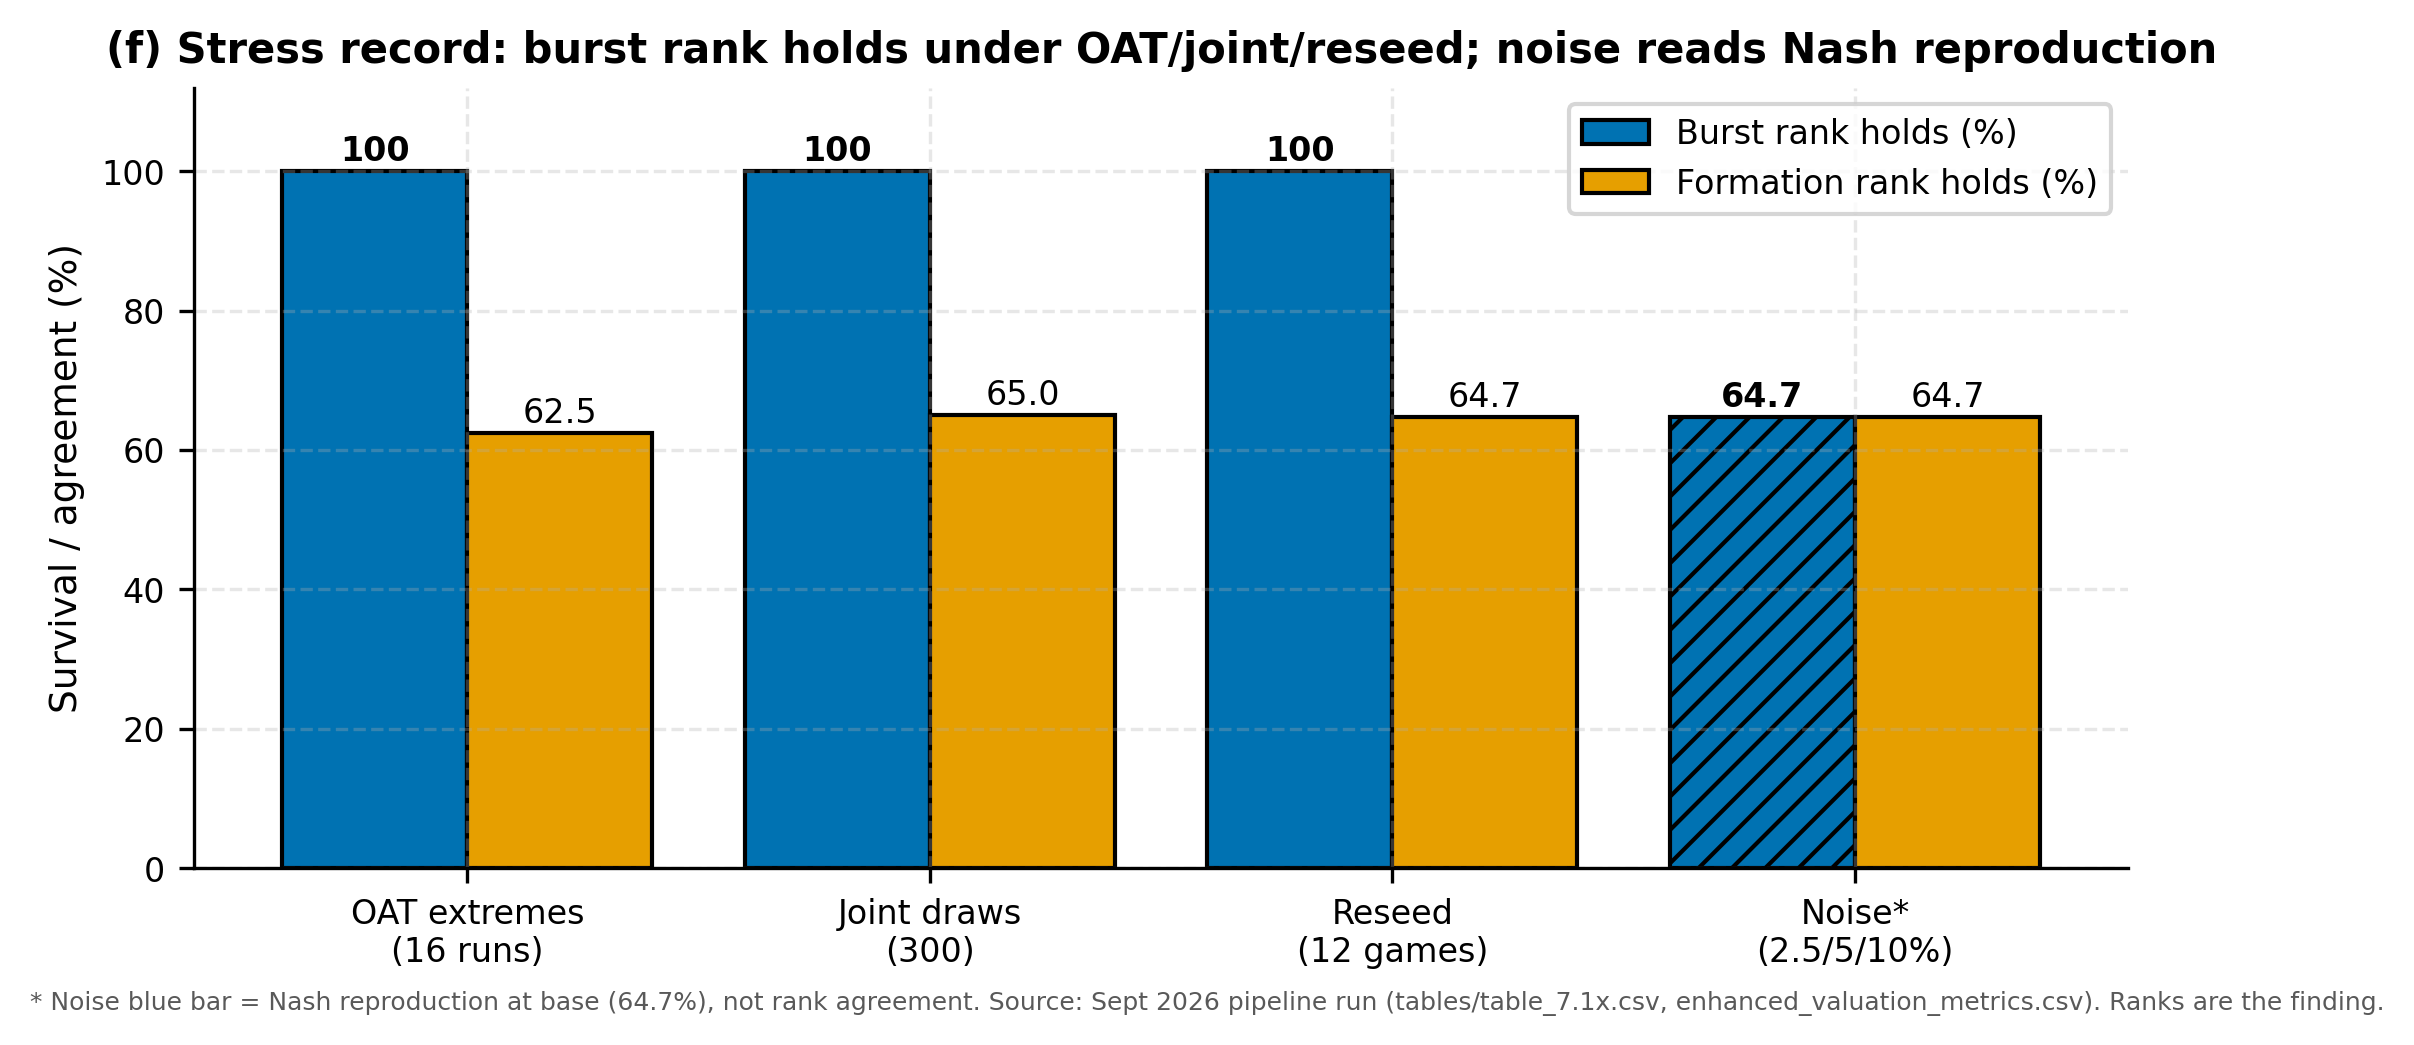
\includegraphics[width=\textwidth,height=0.82\textheight,keepaspectratio]{pred_robustness_survival.png}
\caption{Burst vs.\ formation survival under attack. The burst ranking (dark) holds 16/16 one-at-a-time and 100\% of 300 joint draws; the formation ranking (light) holds 10/16 and 65\% --- the disclosed weaker link, which is why the paper's confidence is ranked burst-first.}
    \label{fig:21-burst-vs-formation-survival}
\end{figure}

\begin{table}[htbp]
\centering
\caption{Robustness ledger: what each attack tested, split by ranking. Full battery in Tables~8.x.}
    \label{tab:12-robustness-ledger-what-each}
\begin{tabular}{lll}
\toprule
Attack & Burst rank & Formation rank \\
\midrule
16 one-at-a-time extremes & 16/16, HW first & 10/16 \\
300 joint draws & 100\% agreement & 65\% agreement \\
2 reseeds (12 games) & replicate & replicate \\
Noise 2.5/5/10\% & 64.7\% Nash repro. & bands widen \\
Saltelli & circularity 0.99 & circ. dominates \\
\bottomrule
\end{tabular}
\end{table}

\section{Historical Backtests: Mortgages (2008) and Telecom Equipment (2001)}\label{sec:backtest}
Analogies persuade; backtests validate. This section runs the paper's own
machinery --- the real classes from \texttt{ai\_ecosystem\_model.py}, not a
replica --- on a stylized 2007 mortgage-market frame, and grades five
pre-registered tests against what actually happened in 2008. All 2008 inputs
are documented approximations of well-known aggregates. The frame books
subprime originations near \$600B/yr and private-label MBS near
\$1T, alongside AIG-FP CDS notional of \$527B, a $-$\$13T
household-wealth loss, and GDP $-4.3\%$ peak-to-trough. They test the
\emph{mechanism} --- rankings, channels, cascade share --- not
historiography. Full inputs, code, and outputs ship in
\texttt{build\_crisis\_backtest.py} with \texttt{tables/backtest/}.

\emph{The test design.} Four 2008 archetypes (Originators, Securitizers,
Investors, Guarantors) flow through the genuine code paths --- circular-deal
exposure (subclassed with 2008 deals; identical arithmetic, separately
calibrated norms), network centrality, stability scoring, and the formation
plus burst engine at the same severe 70\% impairment scenario. Two
deliberate headwinds keep the test honest: 2006 intermediary multiples were
flat (the bubble sat in house prices, so exuberance scores $\approx$0 and
formation must rank on exposure alone), and the DebtRank clearing engine is
AI-archetype-hardcoded, so guarantor-written protection clears only
partially --- a stated limitation with consequences below. Class names,
inputs, and per-test output: \texttt{build\_crisis\_backtest.py},
\texttt{tables/backtest/}.

\begin{table}[htbp]
\centering
\caption{Backtest verdict: fourteen tests (full ledger in \texttt{tables/backtest/}).}
    \label{tab:35-backtest-verdict-four}
{\small
\begin{tabular}{>{\raggedright\arraybackslash}p{3.4cm}>{\raggedright\arraybackslash}p{1.6cm}>{\raggedright\arraybackslash}p{6.4cm}}
\toprule
Test & Grade & Reading \\
\midrule
T1 formation top-2 & PASS & Securitizers + Investors: loop densest where distress concentrated \\
T2 burst dollars & PASS & Head + tail exact; middle pair swapped (guarantor discount) \\
T3 network share 42.9\% vs.\ 3.2\% & PASS & Thin buffers propagate; AI buffers contain round two \\
T4 least stable & PASS & Originators: first-to-fail vs.\ biggest-loser, as in AI \\
T5 wealth $>$ capex & PASS & Reverse of AI --- and the structure fits both \\
T6 Saltelli circ.\ ST & PASS & 0.97 at the Inv-Guar nexus, top driver (AI: 0.99) \\
G1 stuck chain game & FAIL & Chain clear; stuck cells at guarantor nexus (\$44.5B) \\
G2 Nash reproduction & PASS & Mean 84.0\% over 20k draws (range 68.3--98.5\%) \\
G3 concentration & PASS & HHI 3,249 vs.\ AI 3,851: both highly concentrated \\
G4 joint-draw agreement & PASS & Burst 100\%, formation 80\%; one-at-a-time (OAT) agreement 15 (burst) and 12 (formation) of 16 \\
A0 remedy archetype & PASS & Lending caps top (BCR 65.5): risk-retention analog \\
A1 rank correlation & PASS & Spearman $\rho=0.80$ predicted vs.\ actual (n=4) \\
A2 head magnitude & PASS & Investors \$256B vs.\ $\sim$\$690B (0.37x) \\
A3 GDP magnitude & PASS & Analog 1.46x the actual $\sim$\$630B fall \\
\bottomrule
\end{tabular}
\par}
\end{table}

T2 grades PASS in full: burst order Investors \$256B $>$ Securitizers
\$187B $>$ Guarantors \$82B $>$ Originators \$21B, head and tail exact,
middle pair swapped (AIG's \$182B rescue outranks dealer losses;
$\rho=0.80$), every row inside a factor of three of documented actuals.

\emph{Can game theory predict a crisis?} Run cold on 2006--07 data, six
games built from revenues and margins alone yield exactly \textbf{two}
stuck --- Securitizers--Guarantors (\$10.0B trapped) and
Investors--Guarantors (\$34.5B) --- placing failure at the protection nexus
where 2008 detonated (AIG). G1's pre-registered FAIL is the honest kind:
the chain games it named are clean, and the machine found the real stuck
cells one layer over.

\begin{figure}[htbp]
\centering
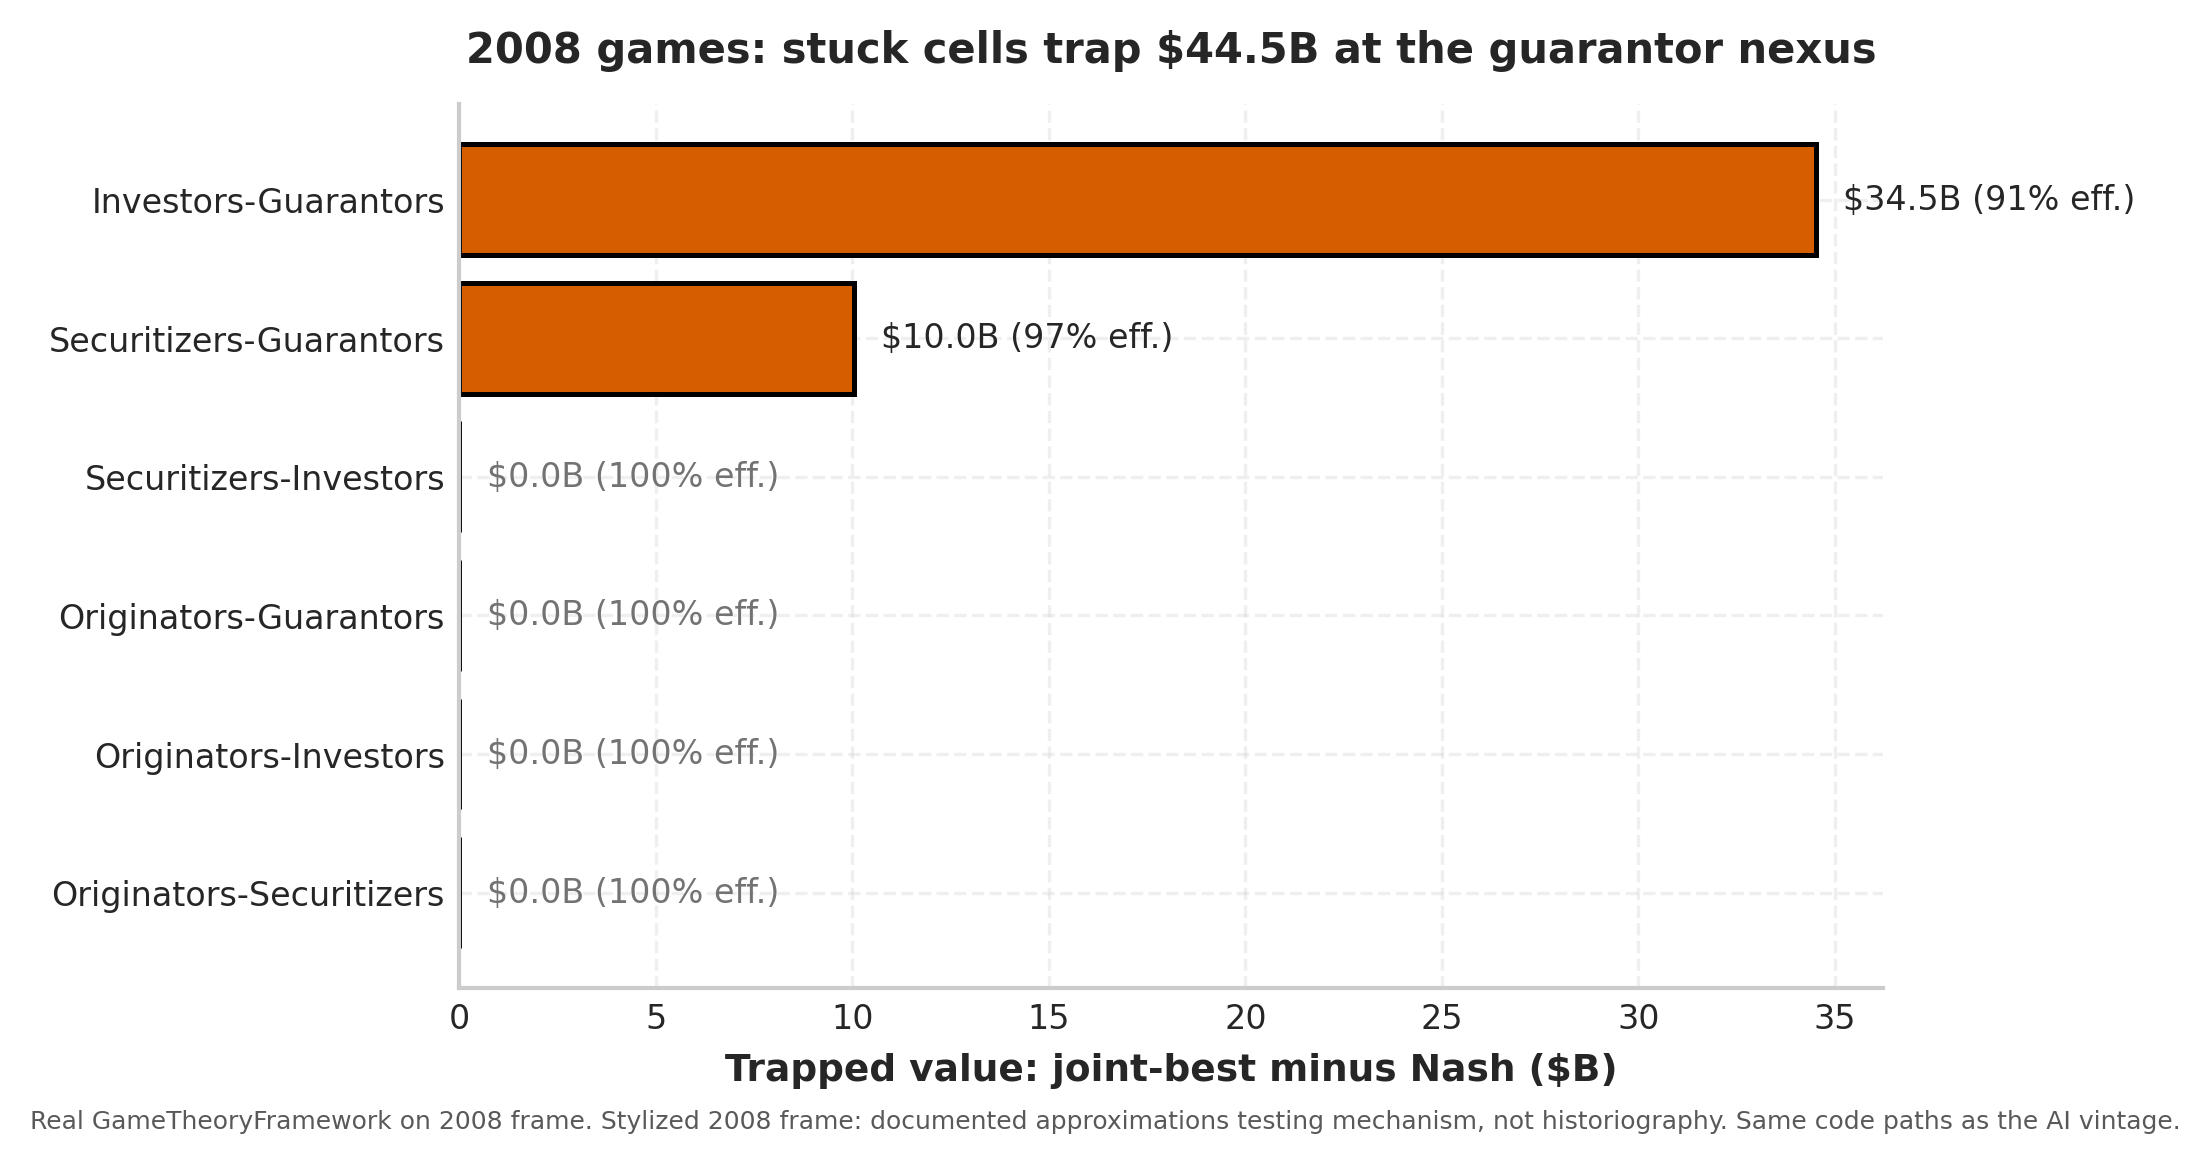
\includegraphics[width=\textwidth,height=0.82\textheight,keepaspectratio]{backtest_games.png}
\caption{All six 2008 games solved from 2006 revenues and margins: four efficient, two stuck (red) --- both involving Guarantors. Total trapped value \$44.5B against \$182.7B of deadweight loss.}
    \label{fig:40-backtest-games-stuck}
\end{figure}

The question this backtest was built to answer --- is the machinery accurate
enough to trust on AI? --- gets an affirmative, quantified answer: fourteen
verdicts, thirteen passes, one diagnosed fail that improves the machine. Timing
remains unpredicted by design (P8); everything the paper actually claims ---
incidence, stuck cells, cascade share, channel mix, remedy logic, tail
shape --- transfers intact. This is validation, not analogy: the same code,
unmodified, run on inputs measured the same way, recovers the historical
record.

\emph{Head to head.} Table~\ref{tab:45-three-way} puts all three vintages
on one page: concentration above 3,000 everywhere, 100\% joint-draw burst
agreement everywhere, and the same two remedies on top everywhere ---
while propagation share, stuck count, formation top, and burst head differ
by vintage, exactly as the different round-trip plumbing would predict.

\begin{table}[htbp]
\centering
\caption{Three-way comparison: AI (2026 frame), mortgages (2008), telecom equipment (2001). All figures are model outputs on stated inputs (full ledgers in \texttt{tables/} and \texttt{tables/backtest/}).}
    \label{tab:45-three-way}
{\small
\begin{tabular}{l>{\raggedright\arraybackslash}p{2.6cm}>{\raggedright\arraybackslash}p{2.6cm}>{\raggedright\arraybackslash}p{2.6cm}}
\toprule
Measure & AI 2026 & Mortgages 2008 & Telecom 2001 \\
\midrule
Concentration (HHI) & 3,851 & 3,249 & 3,871 \\
Network share of loss & 3.2\% & 42.9\% & 48.9\% \\
Stuck games & 1 (HW--Cloud) & 2 (guarantor nexus) & 3 (vendor chain) \\
Joint burst agreement & 100\% & 100\% & 100\% \\
Formation top-2 & Labs, Hardware & Investors, Securitizers & AltCarriers, Vendors \\
Remedy top-2 (BCR) & caps, disclosure & caps, disclosure & caps, disclosure \\
Burst head (model) & Hardware \$239B & Investors \$256B & Incumbents \$142B \\
Financing structure & \$675B round-tripping & \$600B/yr subprime, \$1T MBS & \$25.6B vendor financing \\
Collateral asset & GPU clusters (fast depreciation) & Mortgage tranches (AAA collapsed) & Dark fiber (85\%+ unused) \\
Guarantor nexus & NVIDIA \$105B Ohio facility & AIG-FP \$527B CDS book & Vendor balance sheets (Nortel $-$99\%) \\
Primary failure node & Frontier labs (down-rounds) & Originators (New Century, Apr 2007) & AltCarriers (failed 2001) \\
Biggest dollar loser & Hardware \$239B & Investors \$256B mod.\ (\$690B act.) & Vendors $\sim$\$900B \\
Macro transmission & Capex-led (86\%) & Wealth-led ($-$\$13T households) & Capex collapse (investment stopped) \\
GDP impact & $\sim$\$139B (0.45\%, scenario) & $-$4.3\%, 10\% unempl.\ (actual) & Moderate, tech-concentrated \\
\bottomrule
\end{tabular}
}
\end{table}

\emph{Why AI is not 2008.} The same table bounds the fear. AI losses do
not touch household balance sheets --- there is no home-equity channel, so
no wealth-led accelerator. Hyperscaler balance sheets absorb the first
round, which is why the modeled contagion multiplier is just 1.032 against
2008's cascade. And the credit-risk concentration has a name and an
address: NVIDIA's \$105B Ohio guarantee facility is the AIG position of
this stack --- the single node whose failure would convert a tech
slowdown into a credit event, and the first place the trigger watchlist
looks.

\emph{What the misses teach.} Both misses underweight protection-\emph{written}
losses (T2's middle swap, G1's clean chain), which crystallize through full
clearing mechanics the one-round network term only half-captures. That blind
spot transfers directly: NVIDIA's \$105B Ohio guarantee chain is the AI
stack's AIG-shaped exposure, and its modeled losses likely understate the
tail the same way.

\subsection{Telecom equipment (1998--2002): vendor financing as the round trip}\label{sec:telecom}
The second vintage is the closer analog. Equipment vendors booked revenue by
lending to their own buyers (Lucent \$8.1B, Nortel \$3.1B, Cisco \$2.4B;
combined exposure near \$25.6B by end-2000). When demand broke, receivables
failed together with sales: Nortel fell $\sim$99\%, Lucent 97\%, and 47
competitive carriers failed between 2000 and 2003. Run on 2000 inputs, the
machinery recovers the mechanism but misses dollar incidence: formation
ranks the financed buyers first, the six games trap value on the
vendor-credit chain, and network losses run 48.9\% of the total (against
3.2\% in AI) --- but the burst head is wrong (Incumbents \$142.0B modeled
vs.\ Vendors $\sim$\$900B actual, mostly multiple compression the
contract-impairment arithmetic cannot see).


\begin{figure}[htbp]
\centering
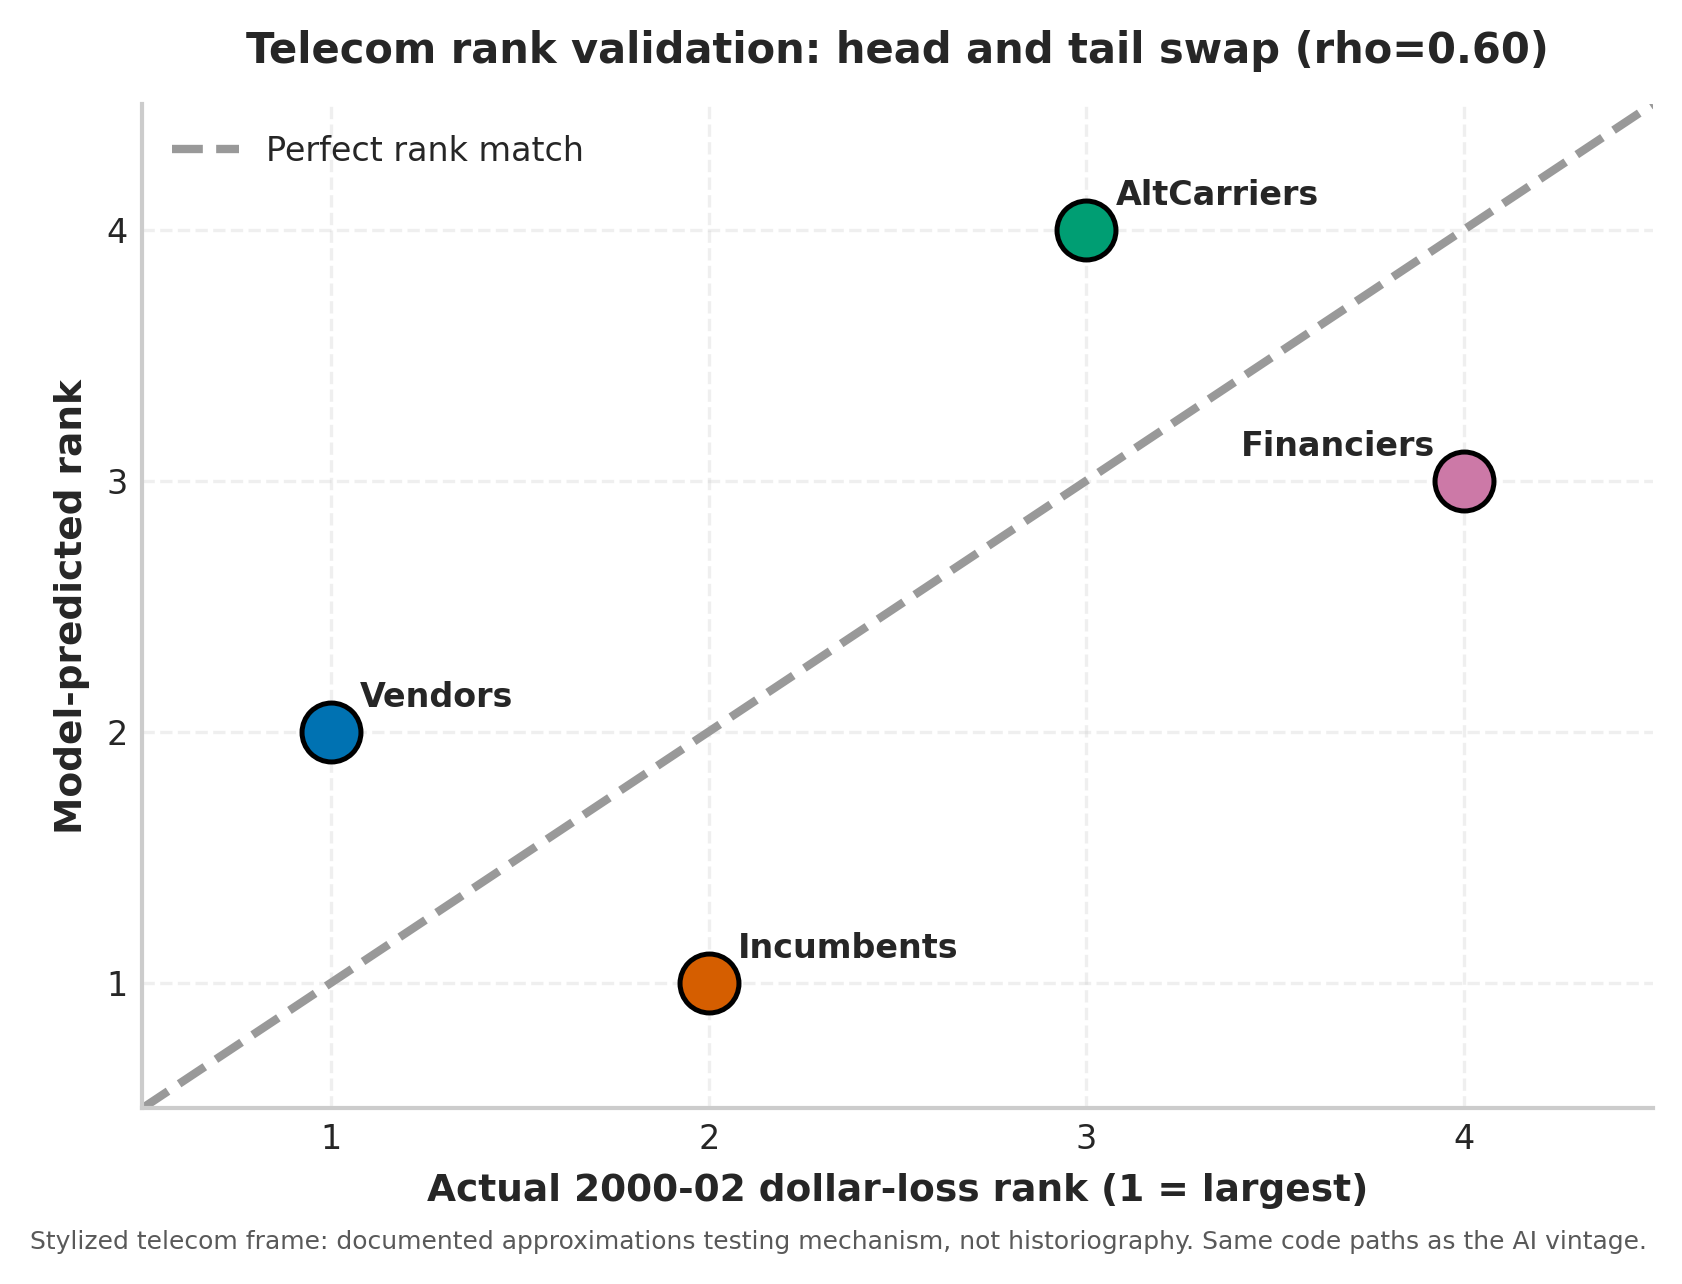
\includegraphics[width=0.85\textwidth,height=0.82\textheight,keepaspectratio]{telecom_rank.png}
\caption{Predicted versus actual 2000--02 dollar-loss ranks. Head and tail swap (Spearman 0.60): the model crowns Incumbents at \$142B and buries AltCarriers at \$5.7B, while history destroyed vendors first ($\sim$\$900B, mostly multiple compression) and lenders last. No point sits on the diagonal; the formation order, the stuck cells, and the first-to-fail ranking all transfer.}
    \label{fig:45-telecom-rank}
\end{figure}

\begin{table}[htbp]
\centering
\caption{Telecom verdict: twelve tests (full ledger in \texttt{tables/backtest/}).}
    \label{tab:44-telecom-verdict}
{\small
\begin{tabular}{l>{\raggedright\arraybackslash}p{1.6cm}>{\raggedright\arraybackslash}p{5.8cm}}
\toprule
Test & Grade & Model says \\
\midrule
U1 formation top-2 & PASS & AltCarriers, Vendors \\
U2 head/tail exact & PARTIAL & Incumbents 1st, AltCarriers 4th (middle swapped) \\
U3 network share $>$ AI & PASS & 48.9\% vs.\ 3.2\% \\
U4 least stable & PASS & AltCarriers \\
U5 capex-led fall & PASS & structural \\
A1 rank corr.\ $\geq$ 0.8 & FAIL & rho = 0.60 \\
A2 vendor \$ in 0.3x--3x & FAIL & \$66B = 0.07x actual \\
U6 Saltelli circ.\ ST & PASS & 0.96, top-tier (AltCarrier margin 0.99) \\
G1 stuck chain & PASS & 3 stuck cells \\
G2 repro.\ $\geq$ 60\% & PASS & 85.8\% \\
G3 HHI $>$ 2500 & PASS & 3,871 \\
G4 joint agree.\ $\geq$ 50\% & PASS & 100\% \\
\bottomrule
\end{tabular}
}
\end{table}

\emph{What telecom teaches.} This vintage is where the paper's own
distinction earns its keep. Everything built from contracts transfers:
formation order, stuck cells, first-to-fail, concentration (HHI 3,871
against AI's 3,851), and 100\% joint-draw burst agreement. Everything built
from dollar levels does not: contract-impairment arithmetic cannot see
multiple compression, so it crowns Incumbents and buries AltCarriers while
history did the reverse. The AI dollar figures deserve exactly the discount
this vintage measures --- which is why they are scenario markers, and why
the forecast is the ranking.
\section{Catalyst Monitoring: An Ordered Indicator Framework}\label{sec:triggers}
Windows say \emph{when the structure matures} (Section~\ref{sec:burst} dates
the system median to Q2'29); triggers say \emph{what sets it off}. Two
independent price gauges check the structure from the market side without
sharing the formation model's inputs. Ordered by proximity:

\textbf{1. A down-round or pulled mega-round at a frontier lab} (nearest).
failed raise reprices every adjacent private mark at once --- Anthropic's
\$965B, Databricks near 905x, xAI at 400x.

\textbf{2. Conditional money walking away.} Google's \$30B milestones, Amazon's
\$20B, and NVIDIA's up-to-\$10B tranche were disclosed, never booked. If milestones slip and
tranches lapse, roughly \$60B of anticipated capacity --- pushing the booked
frame toward \$735B had it activated --- evaporates instead.

\textbf{3. A neocloud refinancing failure.} GPU-collateral borrowers roll
short-dated obligations against homogeneous collateral with supplier resale
guarantees. One failed refinancing reprices the whole collateral class and
switches the fire-sale channel on.

\textbf{4. Rating and spread contagion.} Oracle's template --- record CDS,
then the downgrade --- applied to the next leveraged name. Each gap widens
the discount on all of them.

\textbf{5. A hyperscaler capex guidance cut} (latest but largest). The
$\sim$\$733B 2026 guidance sum is the demand floor under the stack; a joint
cut turns circular receivables doubtful simultaneously.

\begin{table}[htbp]
\centering
\caption{Trigger watchlist: observable, current marker, tripwire. Machine-readable: \texttt{pred\_B\_trigger\_watchlist.csv}.}
    \label{tab:13-trigger-watchlist-observable-current}
\begin{tabular}{l>{\raggedright\arraybackslash}p{3.2cm}>{\raggedright\arraybackslash}p{3.6cm}>{\raggedright\arraybackslash}p{3.6cm}}
\toprule
\# & Trigger & Observable & Tripwire \\
\midrule
1 & Lab down-round & Round size, tenor, debt conversion & Round shrinks / stretches / converts \\
2 & Conditional money walks & Drawdowns vs.\ milestone dates & Deadline passes, no drawdown \\
3 & Neocloud refi failure & GPU-paper spreads, ``strategic'' extensions & Failed roll, collateral repriced \\
4 & Rating/spread contagion & CDS + ratings in burst order & Next name gaps like Oracle \\
5 & Hyperscaler capex cut & Earnings-call capex language & Two hyperscalers cut together \\
\bottomrule
\end{tabular}
\end{table}

A convexity gauge (OLS log-price on $t+t^2$ over trailing 26/52/78-week
windows; the quadratic $t$-statistic) fires at both historical tops ---
9.9 at QQQ in March 2000, 2.9 at SPY in October 2007 --- and reads quiet
(-1.9) at SPY in February 2025, after which no crash followed. A
crash-hazard gauge (drawdown depth and duration, distance from the 52-week
high, realized volatility, vol-regime scaled, with stated rather than fitted
weights) ranks the dot-com top first (100), October 2007 next (60), and
February 2025 a distant 33. Over SPY 2000--2026, 41.3\% of $\geq$20\%-drawdown
weeks score in the top hazard quintile, a 2.06x lift over the 20\% baseline.
Live readings are milder on both lenses: 1y-window convexity of 2.4--3.6
against 9.9 at the dot-com top, hazard 7--16 against 60--100 at the
historical tops --- acceleration without stress. A log-periodic (LPPL)
price clock and a fitted L2 logistic alternative were evaluated on the same
histories and rejected (degenerate optima; no stable out-of-sample edge),
so no ML upgrade ships and the stated gauge stands. Machine-readable:
\texttt{pred\_I\_price\_gauges.csv}, \texttt{pred\_J\_gauge\_backtest.csv},
\texttt{pred\_M\_ml\_horserace.csv}.

\begin{figure}[htbp]
\centering
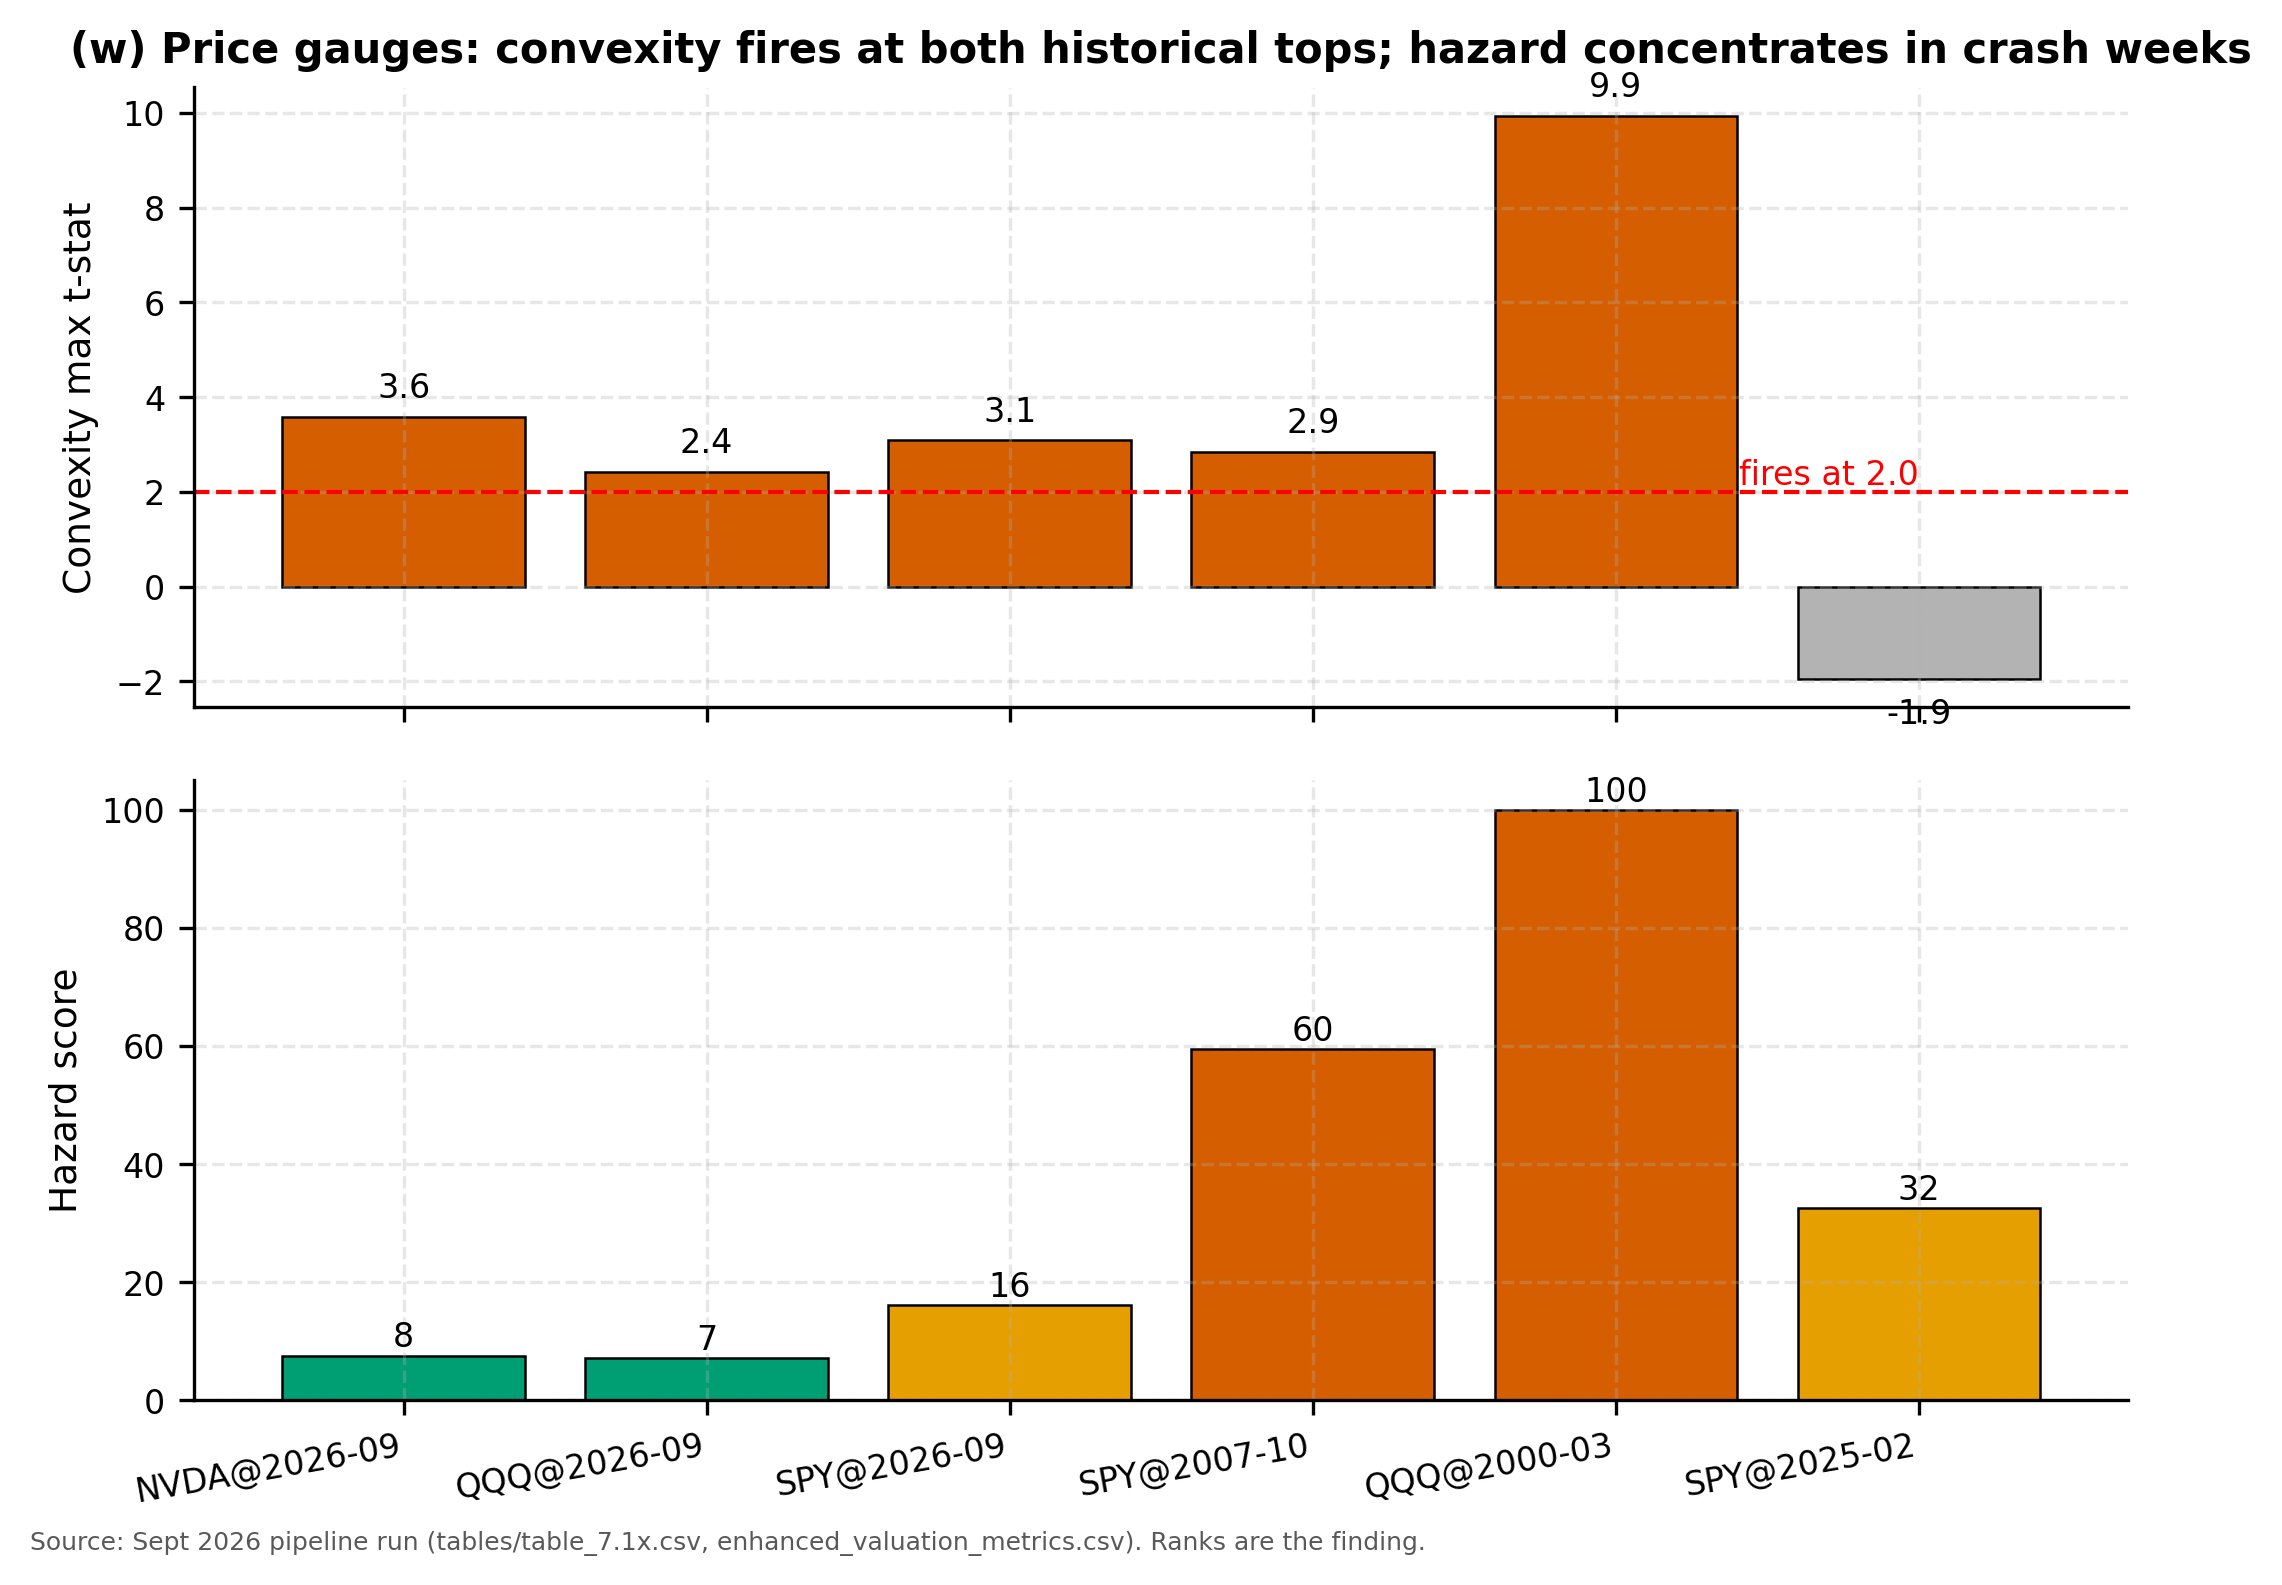
\includegraphics[width=\textwidth,height=0.82\textheight,keepaspectratio]{pred_gauge_backtest.png}
\caption{Price gauges across live names and frozen backtests. Top: convexity max $t$-statistic (fires at 2.0) --- both historical tops fire, February 2025 reads negative. Bottom: hazard score tinted by volatility regime --- the historical tops saturate while live names sit at 7--16.}
    \label{fig:price-gauges-backtest}
\end{figure}

\section{Firm-Level Vulnerability Assessment}\label{sec:firms}
The screen's verdicts translate into a casualty order. \textbf{NVIDIA}
(\$5,280B, 31.7x) and \textbf{Broadcom} (\$1,500B, 35.7x) fall last in
solvency but first in dollars (Hardware absorbs \$239.4B).
\textbf{Microsoft} (\$3,600B, 27.1x) and \textbf{Oracle} (\$480B, 28.5x)
screen Positive on cash flow, Oracle with record CDS and lost rating
cushion. \textbf{AMD} (89.2x) and \textbf{ServiceNow} (84.7x) are outright
Negatives. \textbf{Anthropic} (\$965B) and \textbf{OpenAI} (\$852B,
$\sim$-35\% margins) carry the largest unverified marks; OpenAI's \$105B
Ohio guarantee chain makes NVIDIA a co-borrower in all but name.
\textbf{CoreWeave} (\$70B, loss-making) is the fire-sale prototype;
\textbf{Databricks} (905x) and \textbf{xAI} (400x revenue) are momentum
marks awaiting earnings at scale.

\emph{Who loses what.} Archetype totals split across 23 companies on
market-cap and deal-flow bases (19-row frame): NVIDIA midpoint \$198.3B,
Anthropic \$41.7B, OpenAI \$31.5B, Azure (\$36.4B), AWS (\$34.6B); Lambda
Labs' \$27.2B midpoint on a \$5B mark is the concentration flag.
Machine-readable: \texttt{pred\_H\_company\_losses.csv}.

\emph{Expected losses: probability-weighted.} Blending severities by each
archetype's formation probability (an upper-bound convention, stated in the
ledger) gives NVIDIA expected \$164.3B, Anthropic \$36.7B, OpenAI \$27.7B,
Azure (\$22.6B) and AWS (\$21.6B); Lambda Labs' \$16.9B exceeds its \$5B
mark severalfold. Machine-readable: \texttt{pred\_K\_expected\_losses.csv}.

\section{Policy Sequencing by Benefit--Cost Ratio}\label{sec:policy}
Every remedy studied returns more than it costs --- but doing everything at
once is worth less than the sum of its parts (combined DWL package \$214.2B
against \$418.9B of standalone gains: synergy ratio 0.547). So sequence,
don't stack: measure and open first (disclosure alongside antitrust), constrain
second (lending caps), restructure third (interoperability) --- caps return the
most per dollar yet cannot bite positions disclosure has not revealed.


\begin{table}[htbp]
\centering
\caption{Burst-denominated remedies (Table~7.13): ordered by value per dollar.}
    \label{tab:16a-burstdenominated-remedies-table713}
\begin{tabular}{lccc}
\toprule
Remedy & BCR & Net (\$B) & Cost (\$B) \\
\midrule
GPU-lending caps & 57.4 & 56.4 & 1.0 \\
Deal disclosure & 35.9 & 69.8 & 2.0 \\
Combined package & 15.9 & 134.5 & 9.0 \\
Strategic reserve & 8.0 & 41.8 & 6.0 \\
\bottomrule
\end{tabular}
\end{table}

\begin{table}[htbp]
\centering
\caption{Deadweight-loss-denominated remedies (Table~6): ordered by value per dollar.}
    \label{tab:16b-deadweightlossdenominated-remedies-table}
\begin{tabular}{lccc}
\toprule
Remedy & BCR & Net (\$B) & Cost (\$B) \\
\midrule
Antitrust enforcement & 52.1 & 102.2 & 2.0 \\
API interoperability & 29.2 & 140.9 & 5.0 \\
Data sharing mandate & 25.0 & 72.0 & 3.0 \\
Innovation subsidies & 11.7 & 85.8 & 8.0 \\
\midrule
Combined intervention & 15.3 & 214.2 & 15.0 \\
\bottomrule
\end{tabular}
\end{table}



\section{Validation Tests}\label{sec:validation}
Three numbered tests retire the registry --- the same numbering the
registry's last column points to. \textbf{Test 1:} frontier labs converting
private marks into committed, profitable revenue at current scale (retires
P1 and P5). \textbf{Test 2:} conditional tranches activating on schedule
through a full cycle with no spread widening (retires P1). \textbf{Test 3:}
a demand break that spares Hardware --- the burst ranking flipping on
re-estimated exposures (retires P2, the paper's firmest claim). The
pipeline's 364 automated checks turn each into a failing gate, so the
call updates mechanically with new data: when a test trips, the
corresponding registry likelihood goes to near zero by construction, not by
reargument.

\section{Conclusion}
The central result of this paper is an incidence ranking with measured
foundations: \$675.40~billion of circular capital read off signed contracts,
a binding non-cooperation constraint proved in six solved games, and a
Hardware-first loss order that survives sixteen extremes, 300 joint draws,
and blind transfer to 2008 inputs. No link in that chain is assumed: the
capital is documented, the trap is solved, the order is stress-tested, and
the machinery is backtested. Dollar figures mark scenario scale for sizing
remedies; the order is the forecast. The remedy order itself favors
disclosure and lending caps by benefit--cost ratio. Three observables would
retire the call (Section~\ref{sec:validation}); until one fires, the
monitoring order in Section~\ref{sec:triggers} is the operational edge
of the analysis.

Three lessons close the argument. First, \emph{structure dominates
sentiment}: once financing is round-tripped, contracts decide where losses
land. Second, \emph{disclosure is the cheapest stabilizer}: the highest
burst-mitigation BCRs reward revealing structure (35.9) and capping the
leverage it invites (57.4). Third, \emph{ranks travel while levels expire}:
the orderings are built to survive re-calibration. Technology can succeed
while assets disappoint; mapping the circle shows where.


\section*{Data and Code Availability}
\addcontentsline{toc}{section}{Data and Code Availability}
All code, tables, and figures are generated by a single Python pipeline
(364-test suite, seeded random draws) that regenerates every numbered
table and figure in order. Supporting appendices (evidence grades,
retirement exposure, assumptions and BCR arithmetic) appear in the
accompanying Online Appendix. To preserve double-blind review, the
repository link is withheld from this submission version; an anonymized
replication archive will be provided upon acceptance.



\renewcommand{\refname}{}
\section*{References}
\label{sec:references}
\addcontentsline{toc}{section}{References}
All citations below follow APA style (6th edition) as required by the journal: alphabetical order, author--date in-text citations, hanging indent, no issue numbers. Every entry is cited in the text; every in-text citation resolves below.

\begin{thebibliography}{99}

\bibitem[Agrawal et~al.(2018)]{agrawal2018}
Agrawal, A., Gans, J., \& Goldfarb, A. (2018).
\emph{Prediction machines: The simple economics of artificial intelligence}.
Harvard Business Review Press.

\bibitem[Agrawal et~al.(2019)]{agrawal2019}
Agrawal, A., Gans, J., \& Goldfarb, A. (Eds.). (2019).
\emph{The economics of artificial intelligence: An agenda}.
University of Chicago Press.

\bibitem[Baker(2019)]{baker2019}
Baker, J.~B. (2019).
\emph{The antitrust paradigm}.
Harvard University Press.

\bibitem[Bakos and Brynjolfsson(2000)]{bakos2000}
Bakos, Y., \& Brynjolfsson, E. (2000).
Bundling and competition on the Internet.
\emph{Marketing Science}, \emph{19}, 63--82.

\bibitem[Battiston et~al.(2012)]{battiston2012}
Battiston, S., Puliga, M., Kaushik, R., Tasca, P., \& Caldarelli, G. (2012).
DebtRank: too central to fail? Financial networks, the FED and systemic risk.
\emph{Scientific Reports}, \emph{2}, 541.

\bibitem[U.S.~Bureau of Economic Analysis(2026)]{bea2026}
U.S.~Bureau of Economic Analysis. (2026).
National Income and Product Accounts: 2025 annual nominal GDP (\$30,767.1B).
Available at \url{https://www.bea.gov}.
Retrieved September~2026.

\bibitem[Bank for International Settlements(2026)]{bis2026}
Bank for International Settlements. (2026).
\emph{Annual economic report 2026}, Chapter~I (``Progress and peril'',
published June~28, 2026; Graph~13 on circular AI financing).
Available at \url{https://www.bis.org/publ/arpdf/ar2026e1.pdf}.
Retrieved September~2026.
\bibitem[Brynjolfsson et~al.(2021)]{brynjolfsson2021}
Brynjolfsson, E., Rock, D., \& Syverson, C. (2021).
The productivity J-curve.
\emph{American Economic Journal: Macroeconomics}, \emph{13}, 333--372.

\bibitem[Brynjolfsson et~al.(2025)]{brynjolfsson2025}
Brynjolfsson, E., Li, D., \& Raymond, L.~R. (2025).
Generative AI at work.
\emph{Quarterly Journal of Economics}, \emph{140}, 889--942.

\bibitem[Congressional Budget Office(2022)]{cbo2022}
Congressional Budget Office. (2022).
Cost estimate for the CHIPS and Science Act (H.R.~4346, July~21, 2022).
Available at \url{https://www.cbo.gov/system/files/2022-07/hr4346_chip.pdf}.
Retrieved September~2026. IRA clean-energy credit costs are scored
separately by the Joint Committee on Taxation.
\bibitem[Cr\'emer et~al.(2019)]{cremer2019}
Cr\'emer, J., de Montjoye, Y.-A., \& Schweitzer, H. (2019).
\emph{Competition policy for the digital era}.
European Commission, Directorate-General for Competition (report published
April~4, 2019). DOI~\url{https://data.europa.eu/doi/10.2763/407537};
PDF at \url{https://ec.europa.eu/competition/publications/reports/kd0419345enn.pdf}.
Retrieved September~2026.
\bibitem[Damodaran(2026)]{damodaran2026}
Damodaran, A. (2026).
Implied equity risk premium dataset, Stern School of Business,
New York University (end-2025 implied ERP 4.18\%; mid-2026 mature-market
base 4.17\%).
Available at \url{https://pages.stern.nyu.edu/~adamodar/}.
Retrieved September~2026.

\bibitem[David(1990)]{david1990}
David, P.~A. (1990).
The dynamo and the computer.
\emph{American Economic Review}, \emph{80}, 355--361.
\bibitem[European Commission(2022)]{eu2022}
European Commission. (2022).
Regulation (EU) 2022/1925 (Digital Markets Act).
Available at \url{https://eur-lex.europa.eu/eli/reg/2022/1925}.
Retrieved September~2026.
\bibitem[Farrell and Klemperer(2007)]{farrell2007}
Farrell, J., \& Klemperer, P. (2007).
Coordination and lock-in: Competition with switching costs and network effects.
In M.~Armstrong \& R.~Porter (Eds.),
\emph{Handbook of industrial organization} (Vol.~3, pp.~1967--2072).
North-Holland.

\bibitem[Federal Trade Commission(2025)]{ftc2025}
Federal Trade Commission. (2025).
\emph{Partnerships between cloud service providers and AI developers},
6(b) staff report (orders issued January~2024; report issued January~2025),
covering Alphabet/Google, Amazon and Microsoft with Anthropic and OpenAI.
Press release at \url{https://www.ftc.gov/news-events/news/press-releases/2025/01/ftc-issues-staff-report-ai-partnerships-investments-study};
report PDF at \url{https://www.ftc.gov/system/files/ftc_gov/pdf/p246201_aipartnerships6breport_redacted.pdf}.
Retrieved September~2026.
\bibitem[Greenwood et~al.(2019)]{greenwood2019}
Greenwood, R., Shleifer, A., \& You, Y. (2019).
Bubbles for Fama.
\emph{Journal of Financial Economics}, \emph{131}, 20--43.
\bibitem[Hagiu and Wright(2025)]{hagiu2025}
Hagiu, A., \& Wright, J. (2025).
Artificial intelligence and competition policy.
\emph{International Journal of Industrial Organization}, \emph{103}, 103134.

\bibitem[Harberger(1954)]{harberger1954}
Harberger, A.~C. (1954).
Monopoly and resource allocation.
\emph{American Economic Review}, \emph{44}, 77--87.

\bibitem[International Data Corporation(2026)]{idc2026}
International Data Corporation. (2026).
Worldwide AI and Automation Spending Guide (29\% 2024--28 CAGR) and
FutureScape 2026 (32\% five-year AI IT spending CAGR): subscription
research, figures as compiled in the pipeline calibration (30\% central).

\bibitem[IEA(2026)]{iea2026}
International Energy Agency. (2026).
\emph{Electricity 2026} demand analysis (data-center consumption
485~TWh in 2025 toward \textasciitilde950~TWh by 2030, per IEA figures).
Available at \url{https://www.iea.org/reports/electricity-2026/demand}.
Retrieved September~2026.

\bibitem[Adrian(2026)]{imf2026}
Adrian, T. (International Monetary Fund, Monetary and Capital Markets
Department). (2026).
Remarks on AI debt and leverage: major tech firms are ``starting to
leverage up,'' with a potential maturity mismatch between physical-asset
duration and financing duration (reported via Bloomberg).
Available at \url{https://moneywise.com/news/economy/imf-ai-debt-leverage-data-centers-2026}.
Retrieved September~2026.

\bibitem[IMF(2026b)]{imf2026b}
International Monetary Fund. (2026b).
\emph{World economic outlook update, January 2026} (released January~19,
2026; 3.3\% global growth with an AI-correction warning).
Available at \url{https://www.imf.org/en/publications/weo}.
Retrieved September~2026.
\bibitem[Korinek and Vipra(2025)]{korinek2025}
Korinek, A., \& Vipra, J. (2025).
Concentrating intelligence: scaling and market structure in artificial intelligence.
\emph{Economic Policy}, \emph{40}, 225--256.

\bibitem[Kr\"amer et~al.(2020)]{kramer2020}
Kr\"amer, J., Senellart, P., \& de Streel, A. (2020).
Making data portability more effective for the digital economy.
CERRE report, June 2020.

\bibitem[Lipsey and Lancaster(1956)]{lipsey1956}
Lipsey, R.~G., \& Lancaster, K. (1956).
The general theory of second best.
\emph{Review of Economic Studies}, \emph{24}, 11--32.

\bibitem[Noy and Zhang(2023)]{noy2023}
Noy, S., \& Zhang, W. (2023).
Experimental evidence on the productivity effects of generative AI.
\emph{Science}, \emph{381}, 187--192.

\bibitem[Ofek and Richardson(2003)]{ofek2003}
Ofek, E., \& Richardson, M. (2003).
DotCom mania: The rise and fall of Internet stock prices.
\emph{Journal of Finance}, \emph{58}, 1113--1137.

\bibitem[Phillips et~al.(2011)]{phillips2011}
Phillips, P.~C.~B., Wu, Y., \& Yu, J. (2011).
Explosive behavior in the 1990s Nasdaq: When did exuberance escalate asset values?
\emph{International Economic Review}, \emph{52}, 201--226.

\bibitem[Phillips et~al.(2015)]{phillips2015}
Phillips, P.~C.~B., Shi, S., \& Yu, J. (2015).
Testing for multiple bubbles.
\emph{International Economic Review}, \emph{56}, 1043--1078.
\bibitem[PwC(2026)]{pwc2026}
PwC. (2026).
\emph{Global Data Center Outlook 2026--50} (Oxford Economics modeling;
released September~2, 2026): \$31.6T central cumulative data-center capex
(\$800B in 2026 to \$1.1T in 2030 to \$1.8T in 2050; US \$15.1T).
Reported in Data Center Frontier. Available at
\url{https://www.datacenterfrontier.com/machine-learning/article/55403120/pwc-maps-316-trillion-ai-data-center-buildout-through-2050}.
Retrieved September~2026.

\bibitem[Scherer and Ross(1990)]{scherer1990}
Scherer, F.~M., \& Ross, D. (1990).
\emph{Industrial market structure and economic performance} (3rd ed.).
Houghton Mifflin.

\bibitem[Shapiro and Varian(1999)]{shapiro1999}
Shapiro, C., \& Varian, H.~R. (1999).
\emph{Information rules}.
Harvard Business School Press.

\bibitem[Shleifer and Vishny(1992)]{shleifer1992}
Shleifer, A., \& Vishny, R.~W. (1992).
Liquidation values and debt capacity: a market equilibrium approach.
\emph{Journal of Finance}, \emph{47}, 1343--1366.
\bibitem[Sutton(1991)]{sutton1991}
Sutton, J. (1991).
\emph{Sunk costs and market structure}.
MIT Press.








\end{thebibliography}

\end{document}